% =============================================================================
% Small Open-Weight LLMs for Security Tool Use (multi-model benchmark)
% IEEE two-column conference format (IEEEtran, conference mode)
%
% HOW TO COMPILE:
%   Overleaf (recommended): create a project, upload this .tex file AND the
%   images/ folder next to it (same relative path), then Recompile.
%   Local: pdflatex paper.tex   (run twice so citation numbers settle)
%
% STATUS: agent numbers come from RedBlue-MultiAgent/RESULTS.md; CyberMetric,
% Heretic and BFCL numbers come from the multi-model benchmark runs. The agent
% system has five agents (Safety, Orchestrator, Evaluator, Recon,
% Vulnerability Analysis).
% =============================================================================

\documentclass[conference]{IEEEtran}
\IEEEoverridecommandlockouts

\usepackage{cite}
\usepackage{amsmath}
\usepackage{amssymb}
\usepackage{algorithm}
\usepackage{algorithmic}
\usepackage{graphicx}
\usepackage{textcomp}
\usepackage{booktabs}
\usepackage{array}
\usepackage{multirow}
\usepackage{xcolor}
\usepackage{url}

\graphicspath{{images/}}

\def\BibTeX{{\rm B\kern-.05em{\sc i\kern-.025em b}\kern-.08em
    T\kern-.1667em\lower.7ex\hbox{E}\kern-.125emX}}

\begin{document}

\title{Small Open-Weight LLMs for Security Tasks:\\
Knowledge, Tool Calling, Refusal Removal, and an Agent Case Study}

\author{
\begin{minipage}[t]{0.32\textwidth}
\centering
1\textsuperscript{st} D. Vijay Anand\\
\textit{Assistant Professor}\\
\textit{Department of Information Technology}\\
\textit{Kongu Engineering College}\\
\textit{Project Guide}\\
{\small erovijay@kongu.ac.in}
\end{minipage}%
\hfill
\begin{minipage}[t]{0.32\textwidth}
\centering
2\textsuperscript{nd} Santhosh V\\
\textit{Department of Information Technology}\\
\textit{Kongu Engineering College}\\
{\small santhoshradhai2005@gmail.com}
\end{minipage}%
\hfill
\begin{minipage}[t]{0.32\textwidth}
\centering
3\textsuperscript{rd} Rupesh K R\\
\textit{Department of Information Technology}\\
\textit{Kongu Engineering College}\\
{\small ramalingamrupesh6@gmail.com}
\end{minipage}
}

\maketitle

\begin{abstract}
Most research on AI for cybersecurity uses huge models behind paid services.
Students and small teams usually have one graphics card and a mid-sized open
model, so we tested what such a model can really do. First, we quizzed six
open models on up to 10{,}180 cybersecurity questions; the best scored about
87--88 out of 100. Second, many people use free tools to strip a model's safety
refusals, the moments when it says no to a risky request. We used one such
tool, Heretic, which edits a model's internal weights, tries many settings (we
ran 400), and reports how many requests the edited model still refuses and how
far it has drifted from the original. We took the setting with the fewest
refusals. It cut gpt-oss-20b's refusals from all 100 test requests to 27 (on the
requests it was tuned on), yet its quiz score barely moved: two modified copies
stayed within 0.2 points of the original. Third, on three categories of a
standard tool-use test (simple calls, choosing among several tools, and
knowing when no tool is needed) the model scored 85--89\%. Finally, as a case
study, we placed the model in a small team of AI ``agents'' that look up
software vulnerabilities, with a checker that accepts a claim only if the tool
output shows where it came from. On 50 vulnerabilities the model alone was
already right 99\% of the time. The checker, in its default form, accepted an
answer in only 11\% of runs, because it saw too little of what the agent had
found. Showing it everything raised that to 99\% with no wrong answer accepted.
It checks where a claim comes from, not whether it is true, so we could not
show that it improves accuracy.
\end{abstract}

\begin{IEEEkeywords}
large language models, small language models, cybersecurity benchmarks,
CyberMetric, function calling, refusal removal, abliteration,
evidence grounding, provenance checking, Model Context Protocol
\end{IEEEkeywords}

% =============================================================================
\section{Introduction}
\label{sec:intro}

Getting an LLM to drive offensive-security tooling on its own is no longer a
speculative idea. PentestGPT~\cite{pentestgpt} showed that a GPT-4-class
model, organized around a three-module Reasoning/Generation/Parsing
architecture and supervised by a human operator who actually types the
suggested commands, can make real progress through HackTheBox-style
penetration tests. Since then, researchers have pushed the same basic idea
into autonomous Linux privilege escalation~\cite{happe2026}, memory-and-RAG
driven pentesting assistants~\cite{alsabbagh2026}, and broader surveys of
what generative AI changes about offensive security~\cite{hilario2024}.
Most of that work evaluates whole systems. Much less is known about the
small open-weight models a student or a small team would actually run: how
much security knowledge they hold, whether they can call tools, and what
happens to them when their refusal behavior is reduced, as many
practitioners now do.

This paper is a measurement study of small open-weight models for security
tasks. Its core is three measurements: security knowledge, tool calling,
and the capability cost of reducing refusals. The agent system is a case
study of how one of these models behaves inside a loop with a provenance
check; it is not a fourth pillar and no claim about its effectiveness is made.

\subsection{Problem Statement}
\label{sec:problem}

Most systems above assume a reasoning tier---GPT-4 or comparable, with a
local Llama~3 in the study of~\cite{happe2026} as an exception---that a
great many practitioners, students, and independent researchers simply
cannot run: either it is behind a paid API they cannot afford to call at
scale, or it is not something they can self-host at all. At the same time, a
separate and independent trend has produced standardized tool-calling
infrastructure for LLM agents regardless of model tier: the Model Context
Protocol (MCP)~\cite{mcp-spec} gives an LLM orchestrator a common way to
discover and invoke external tools, and open-source MCP servers already
expose large, real tool catalogs to any MCP-compatible agent.

That leaves open, practically important questions, which this paper
answers with measurements rather than assumption. \textbf{How well do
8--20 billion parameter open-weight models know security material, and do
they differ much from one another? What does it cost a model's capability to
reduce its refusal behavior, as many practitioners do with community
tools? Can such a model call tools correctly? And when it is placed inside a
multi-step agent with no human relaying commands, what goes wrong and can
the failures be caught cheaply?}

\subsection{Contributions}

\begin{enumerate}
\item A six-model comparison on all four CyberMetric sets (80, 500, 2{,}000
  and 10{,}180 questions) with Wilson 95\% confidence intervals and a
  results matrix (Section~\ref{sec:multimodel}). The matrix includes a
  general-purpose reasoning model, a thinking model, a security-specialized
  model, and the unmodified and refusal-reduced forms of gpt-oss-20b.
\item A measurement of the capability cost of refusal reduction. Using the
  Heretic optimizer~\cite{heretic}, we report the refusal-versus-KL-divergence
  frontier (original model: 100/100 refusals) and show with paired exact
  McNemar tests that neither Heretic variant (the reference result and our own)
  differs significantly from the unmodified model on 10{,}180
  questions (Section~\ref{sec:refusal}).
\item A tool-calling check on the Berkeley Function Calling
  Leaderboard~\cite{bfcl} (simple, multiple and irrelevance categories),
  stating which categories were left out and why
  (Section~\ref{sec:bfcl}).
\item A case study: a working five-agent system built as a LangGraph state machine
  (Safety, Orchestrator, Recon, Vulnerability Analysis and Evaluator; one
  local 20B model, one external subprocess), with an evidence-grounding
  Evaluator that accepts only claims supported by captured tool output.
  Across eight end-to-end runs on real CVEs it rejected 12 of 17 findings
  in five runs; the claims rejected in the three runs that ended without
  a verified answer were true per NVD and CISA KEV, so the check is
  reported as a provenance check, with its false-rejection cost stated and compared with no check on 50 held-out CVEs
  (Sections~\ref{sec:approach} and~\ref{sec:testing}).
\item A failure taxonomy of five bugs and infrastructure failures found
  while building and testing the system, each confirmed with a
  before/after re-run (Table~\ref{tab:failures}).
\end{enumerate}

\subsection{Paper Organization}

Section~\ref{sec:terminology} fixes terminology. Section~\ref{sec:related}
positions this work against prior LLM-security systems. Section~\ref{sec:scope}
states the research questions. Section~\ref{sec:approach} describes the
agent system: the graph, the tool surface, the local knowledge base and the
evidence-grounding mechanism. Section~\ref{sec:testing} reports the agent
benchmarks. Section~\ref{sec:multimodel} reports the multi-model comparison
on CyberMetric, the effect of refusal removal, and the tool-calling
results. Sections~\ref{sec:limitations} and~\ref{sec:testing-limitations}
state limitations, Section~\ref{sec:ethics} addresses ethical scope, and
Section~\ref{sec:conclusion} concludes.

% =============================================================================
\section{Terminology}
\label{sec:terminology}

\textbf{LLM agent.} An LLM run in a loop where, at each turn, the model
either gives a final answer or asks to invoke an external \emph{tool},
receives the tool's result back into its context, and continues. The
agents in this paper use penetration-testing and threat-intelligence tools.

\textbf{Tool calling / function calling.} The mechanism by which an LLM's
output is parsed, or for models with native structured output, directly
constrained, into a request to invoke a specific named tool with specific
arguments, rather than being left as free-text prose.

\textbf{Model Context Protocol (MCP)~\cite{mcp-spec}.} A standardized
client-server protocol by which an \emph{MCP host} (the orchestrator
embedding the LLM) discovers and invokes tools exposed by one or more
\emph{MCP servers}, independent of the underlying model or orchestrator
implementation.

\textbf{In-process tool.} A tool implemented as a plain function inside the
same Python process as the agent, with no subprocess, no separate server,
and nothing to orphan on a crash---contrasted in this paper with an MCP
tool, which runs as an independent, separately launched process.

\textbf{Evidence grounding.} A verification step, independent of the model
being evaluated, that only accepts a claim (``the vulnerability is
present,'' ``the task is complete'') as true if it is a verifiable match
against real, previously captured tool output---rather than trusting the
model's self-report.

\textbf{Stall detection.} A safety mechanism in the Orchestrator that
tracks whether repeated dispatch of the same specialist is producing new,
verified progress; if not, after a fixed number of unproductive repeats, the
Orchestrator forces the run to end rather than looping indefinitely.

\textbf{Retrieval-Augmented Generation (RAG).} Injecting relevant retrieved
reference text---in this paper, entries from local security knowledge
bases and reference papers---into the model's context at inference time,
instead of relying solely on what the model already learned during
training.

% =============================================================================
\section{Related Work}
\label{sec:related}

\textbf{PentestGPT~\cite{pentestgpt}} is the reference architecture this
paper re-tests at a different model tier: a Reasoning module that tracks a
pentesting task tree, a Generation module that produces concrete commands,
and a Parsing module that folds tool output back into the tree, with a
human operator executing every suggested command against real
HackTheBox/VulnHub machines. In that setup the human operator is the one
who notices when a suggested step did not actually work. The Evaluator in
this paper (Section~\ref{sec:grounding}) takes over a narrow part of that
job: instead of trusting the model's own claim that a step succeeded, it
requires the claim to be traceable to real, previously captured tool
output.

\textbf{Happe et al.~\cite{happe2026}} (the work behind the hackingBuddyGPT
framework) study autonomous Linux privilege escalation with a narrow,
cleanly binary-scoreable outcome per attempt, and report results for a
fully local, no-human-in-the-loop open-weight model (Llama3) alongside
GPT-3.5-Turbo and GPT-4-Turbo. Their local-model condition is the closest
published setting to this paper's ``no human, one local GPU'' condition,
although the tasks differ (Section~\ref{sec:comparison}).

\textbf{Al-Sabbagh et al.~\cite{alsabbagh2026}} propose Autosecagent, which
combines recursive memory with real-time retrieval-augmented generation for
semi-automated penetration testing under human oversight. This paper treats
RAG as one tool among several, but the two
systems differ in how RAG is used: Autosecagent's RAG pulls live data from
external feeds (NVD, CVE) at run time, whereas this paper's RAG tool
(Section~\ref{sec:rag}) deliberately indexes a static, offline local corpus,
so that its correctness and its failure modes (falling back correctly when
the corpus does not cover a query) can be measured without depending on a
live external service's availability during testing.

\textbf{Hilario et al.~\cite{hilario2024}} survey the risks and open
questions of generative AI in penetration testing at a conceptual level;
this paper is best read as an empirical companion to that survey, offering
measured failure data rather than a further conceptual
discussion.

\textbf{Purple Llama / CyberSecEval~\cite{purplellama}} sets a methodology
for benchmarking LLM cybersecurity risk and capability responsibly. This
paper follows the same scoping discipline when deciding what is and is not
measured or elicited (Section~\ref{sec:ethics}): the goal throughout is
measuring \emph{tool-use reliability and its verifiability}, not eliciting
or publishing novel offensive capability.

\subsection{Positioning: what this paper adds}
\label{sec:related-comparison}

None of the works above report how often a claimed success was checked
against captured tool output and rejected. PentestGPT and hackingBuddyGPT
both report whether a task succeeded; neither reports a check of that kind.
This paper reports one for the implemented system, as a provenance check:
in eight development runs the Evaluator rejected 12 of 17 findings, and in
the three runs that ended without a verified answer the rejected claims
were true (Section~\ref{sec:rq3-practice}). On 50 held-out CVEs we compare it
with no check (Section~\ref{sec:onoff}); the unchecked baseline was already
correct in 99.3\% of runs, so we show its cost and behaviour, not an accuracy gain.

% =============================================================================
\section{Scope}
\label{sec:scope}

\subsection{Research Questions}

\textbf{RQ1 (Reliability).} How reliably does an open-weight LLM in the
8--20B range invoke tools correctly---right name, right arguments, actually
invoked---both on a public tool-calling benchmark and when driving a
multi-agent loop against a real tool surface?

\textbf{RQ2 (Failure taxonomy).} What distinct, reproducible failure modes
occur, and are they attributable to the model, the surrounding agent code,
or the environment the whole system runs on?

\textbf{RQ3 (Behaviour of a provenance check).} What does an
evidence-grounding check, which accepts a claim only if it is traceable to
captured tool output, reject in a small-model agent; what does that cost in
answered runs; and does it change the accuracy of the accepted claims compared
with no check?

\textbf{RQ4 (Progression, secondary).} How far through a staged
reconnaissance-and-analysis task does the system get autonomously before
either completing or safely stalling, and where does it stall?

\textbf{RQ5 (Model comparison).} How do small open-weight models---%
general-purpose, thinking, and security-specialized---compare on a
standard security-knowledge benchmark, and which of the differences are
larger than statistical noise?

\textbf{RQ6 (Cost of refusal reduction).} When a community tool reduces a
model's refusal behavior, how much does accuracy on a knowledge-recall
benchmark change?

\subsection{What the implemented system covers}

This report covers a working five-agent system: three control
agents---a deterministic Safety gate, an LLM Orchestrator/router, and an
evidence-grounding Evaluator---and two tool-using red-team specialists,
Recon and Vulnerability Analysis (Fig.~\ref{fig:phase1},
Table~\ref{tab:agents}). RQ1--RQ4 are addressed for this
subset in Section~\ref{sec:testing}; RQ4 has only a partial answer, bounded
by how far the implemented subgraph can currently go (Safety
$\rightarrow$ Orchestrator $\rightarrow$ \{Recon, Vulnerability Analysis\}
$\rightarrow$ Evaluator $\rightarrow$ end). RQ1 (public benchmark part),
RQ5 and RQ6 are addressed in Section~\ref{sec:multimodel}.

\subsection{Out of Scope (for this report)}

The agent system performs reconnaissance and vulnerability analysis on
public CVE data. It does not exploit, plan attacks, or handle logs or
incidents. The
agent is run only with the base gpt-oss-20b model, so the refusal-reduced
variants are evaluated on benchmarks (Section~\ref{sec:multimodel}) but not
inside the agent. No live, third-party, or unauthorized target is used
anywhere in this work.

% =============================================================================
\section{Approach}
\label{sec:approach}

\subsection{System Overview}

Fig.~\ref{fig:phase1} shows the implemented system, which every benchmark
in Section~\ref{sec:testing} exercises. A Safety gate checks the objective
first. An Orchestrator then routes to one of two red-team specialists, and
every specialist's output passes through a single shared Evaluator before
being counted as verified. The graph is Safety $\rightarrow$ Orchestrator
$\rightarrow$ \{Recon, Vulnerability Analysis\} $\rightarrow$ Evaluator,
looping back to the Orchestrator on an unverified claim and terminating
either on a verified answer or on the stall-limit safety valve described in
Section~\ref{sec:stall}.

\begin{figure*}[t]
\centering
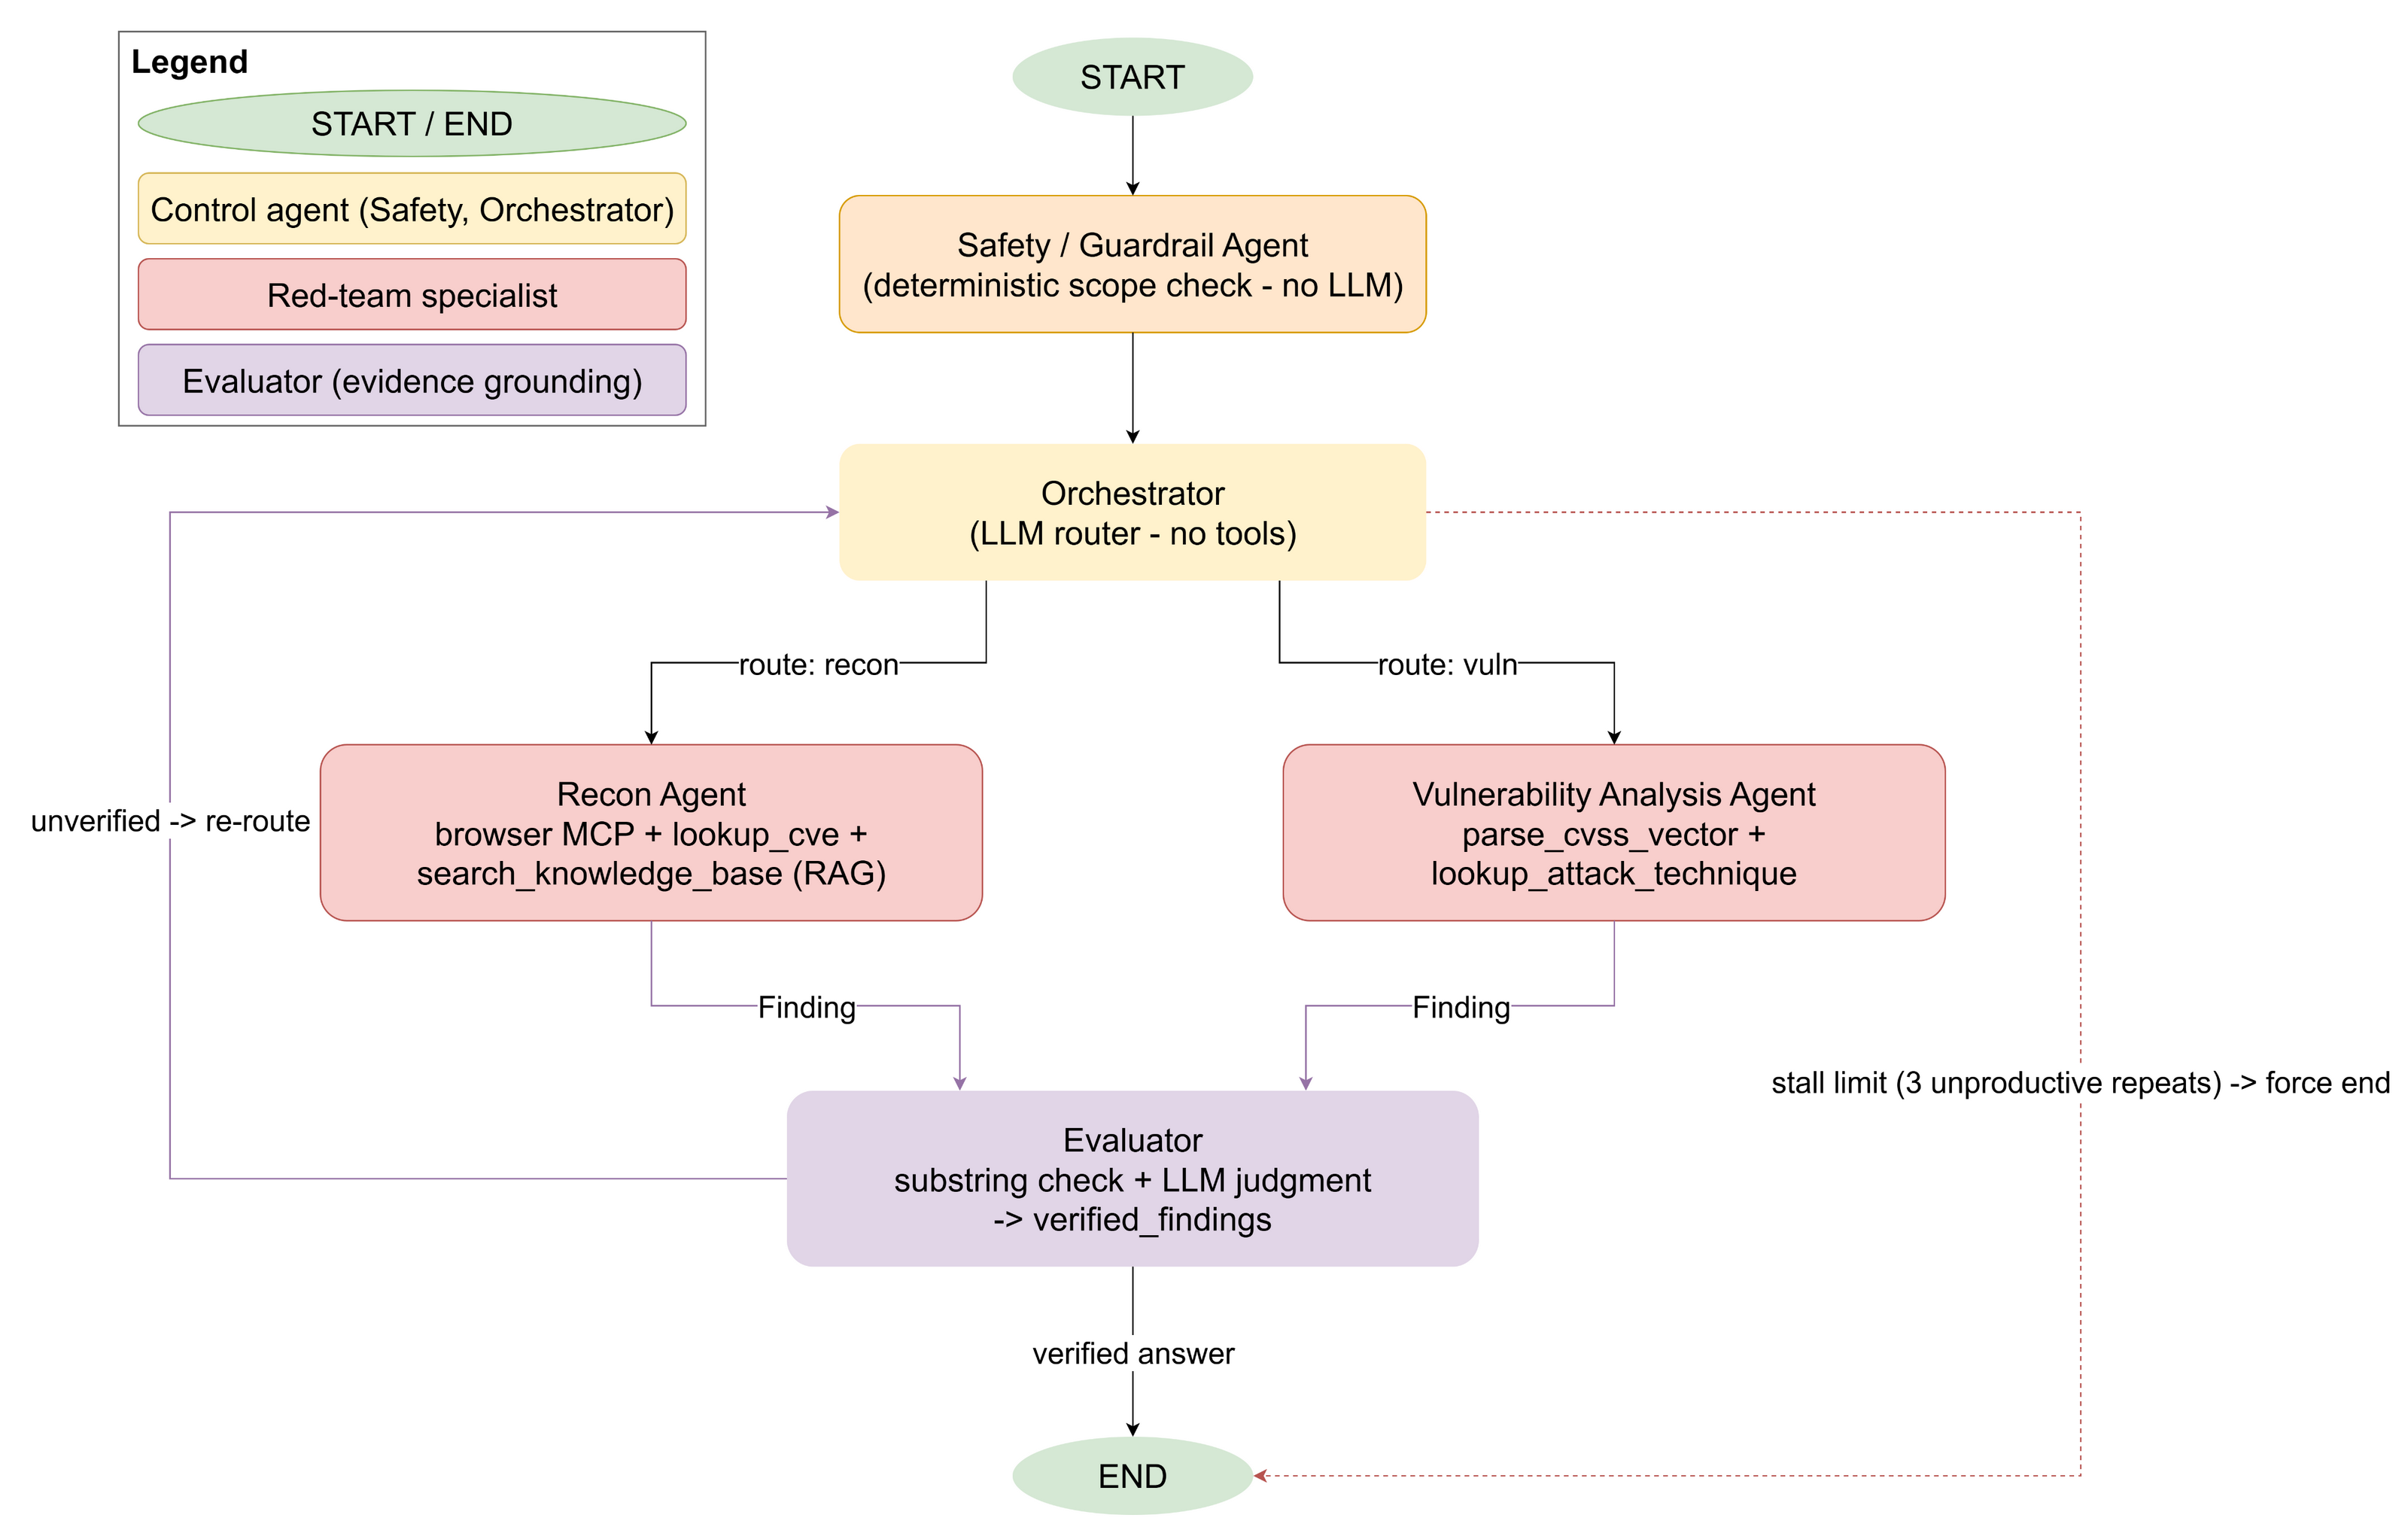
\includegraphics[width=0.8\textwidth]{architecture_implemented.png}
\caption{The implemented five-agent StateGraph, which every agent benchmark
in Section~\ref{sec:testing} exercises. The Safety gate runs first, the
Orchestrator routes to Recon or Vulnerability Analysis, and every finding
passes through the Evaluator. An unverified claim routes back to the
Orchestrator; three unproductive re-dispatches of the same specialist
without new verified progress trip the stall-limit safety valve, and the
Orchestrator forces the run to end rather than loop indefinitely.}
\label{fig:phase1}
\end{figure*}

\subsection{The five implemented agents}
\label{sec:agents}

Table~\ref{tab:agents} lists what each implemented agent does and which tools
it can reach. Three agents form the control plane and two are specialists.
Only Recon touches the browser.

\begin{table*}[t]
\caption{The Five Implemented Agents}
\label{tab:agents}
\centering
\begin{tabular}{@{}llp{4.2cm}p{6.0cm}@{}}
\toprule
\textbf{Agent} & \textbf{Kind} & \textbf{Role} & \textbf{Tools and mechanism} \\
\midrule
Safety & Control, deterministic & Scope allow/deny check on the objective before anything runs & Keyword rules; no LLM call \\
Orchestrator & Control, LLM router & Picks the next specialist or ends the run; tracks stalls (Section~\ref{sec:stall}) & Structured output; no tools \\
Recon & Specialist (red team) & OSINT and CVE lookup & Browser (MCP), NVD API, local knowledge-base search \\
Vulnerability Analysis & Specialist (red team) & CVSS scoring and ATT\&CK technique lookup & \texttt{parse\_cvss\_vector}, \texttt{lookup\_attack\_technique}; no browser \\
Evaluator & Control, two-tier judge & Accepts a claim only if grounded in captured tool output (Section~\ref{sec:grounding}) & Substring check, then a separate LLM judgment \\
\bottomrule
\end{tabular}
\end{table*}

The same five agents exist in two code bases of the project. The benchmark
code in this paper runs against RedBlue-MultiAgent. A second code base wraps
the agents in a Gradio application in which each agent has its own page in
the sidebar, and in which the agents also run together in the RedBlue
Investigate pipeline. The numbers reported in this paper come from
RedBlue-MultiAgent.

\subsection{Why only one subprocess}
\label{sec:subprocess}

Every tool in this system except one is a plain in-process Python function
decorated as a LangChain tool---CVE lookup against the live NVD API, CVSS
vector parsing, local MITRE ATT\&CK lookup, and local knowledge-base search
all run inside the same process as the agent, with no separate server to
launch, monitor, or clean up after a crash. The one exception is browser
automation, exposed through a single MCP server (\texttt{cloakbrowser-mcp})
shared by every browser-needing agent. This was a deliberate trade-off made
under a hard project deadline, motivated by a real, previously encountered
problem: an MCP server launched over a stdio subprocess can silently orphan
its child process tree if the parent is killed, blocking every subsequent
run until the orphan is found and killed by hand. Concentrating that risk
into exactly one subprocess, rather than one per capability, means only one
piece of the system needs a cleanup wrapper (\texttt{run\_agent.sh}) and
only one piece of the system was capable of producing the interop failure
documented in Table~\ref{tab:failures}, row 4. Table~\ref{tab:tools}
inventories every tool actually available to the implemented agents.

\begin{table}[t]
\caption{Tool Inventory}
\label{tab:tools}
\centering
\begin{tabular}{@{}p{2.0cm}p{1.0cm}p{1.7cm}p{2.9cm}@{}}
\toprule
\textbf{Tool} & \textbf{Type} & \textbf{Subprocess?} & \textbf{Backing data} \\
\midrule
\texttt{browser\_*} \newline (26 tools) & MCP server & \textbf{Yes---the only one} & Live web, via cloakbrowser-mcp \\
\texttt{lookup\_cve} & In-process & No & Live NVD REST API \\
\texttt{parse\_\allowbreak cvss\_\allowbreak vector} & In-process & No & \texttt{cvss} library (deterministic; all of v2/v3.0/v3.1/v4.0) \\
\texttt{lookup\_\newline attack\_\newline technique} & In-process & No & Local MITRE ATT\&CK knowledge base \\
\texttt{search\_\newline knowledge\_\newline base} & In-process & No & Local BM25 index, 6{,}713 chunks (Section~\ref{sec:rag}) \\
\bottomrule
\end{tabular}
\end{table}

\subsection{Locally hosted retrieval-augmented knowledge base}
\label{sec:rag}

The Recon agent's system prompt tells it to check a local knowledge base
before reaching for the browser. That knowledge base is a single BM25
keyword index (\texttt{rank\_bm25}) built over 6{,}713 text chunks drawn
from six structured security knowledge bases---MITRE ATT\&CK, CWE, CAPEC,
D3FEND, the CISA Known Exploited Vulnerabilities catalog, and the OWASP
Cheat Sheet series---plus four reference papers (parsed with
Docling~\cite{docling}) and this project's own internal documentation.
BM25 keyword search was chosen over an embedding-based vector index for a
specific, deliberate reason: this corpus is unusually dense with exact
identifiers (\texttt{CVE-2021-44228}, \texttt{T1059.001}), which a general
embedding model's subword tokenizer tends to fragment, hurting nearest-neighbor
retrieval precisely on the tokens that matter most; a keyword index has no
such failure mode, needs no GPU or vector database of its own, and is
trivially fast to query. Fig.~\ref{fig:rag-pipeline} shows the ingestion
pipeline; the resulting index is exposed to any agent as a single shared
tool, \texttt{search\_knowledge\_base}.

\begin{figure}[t]
\centering
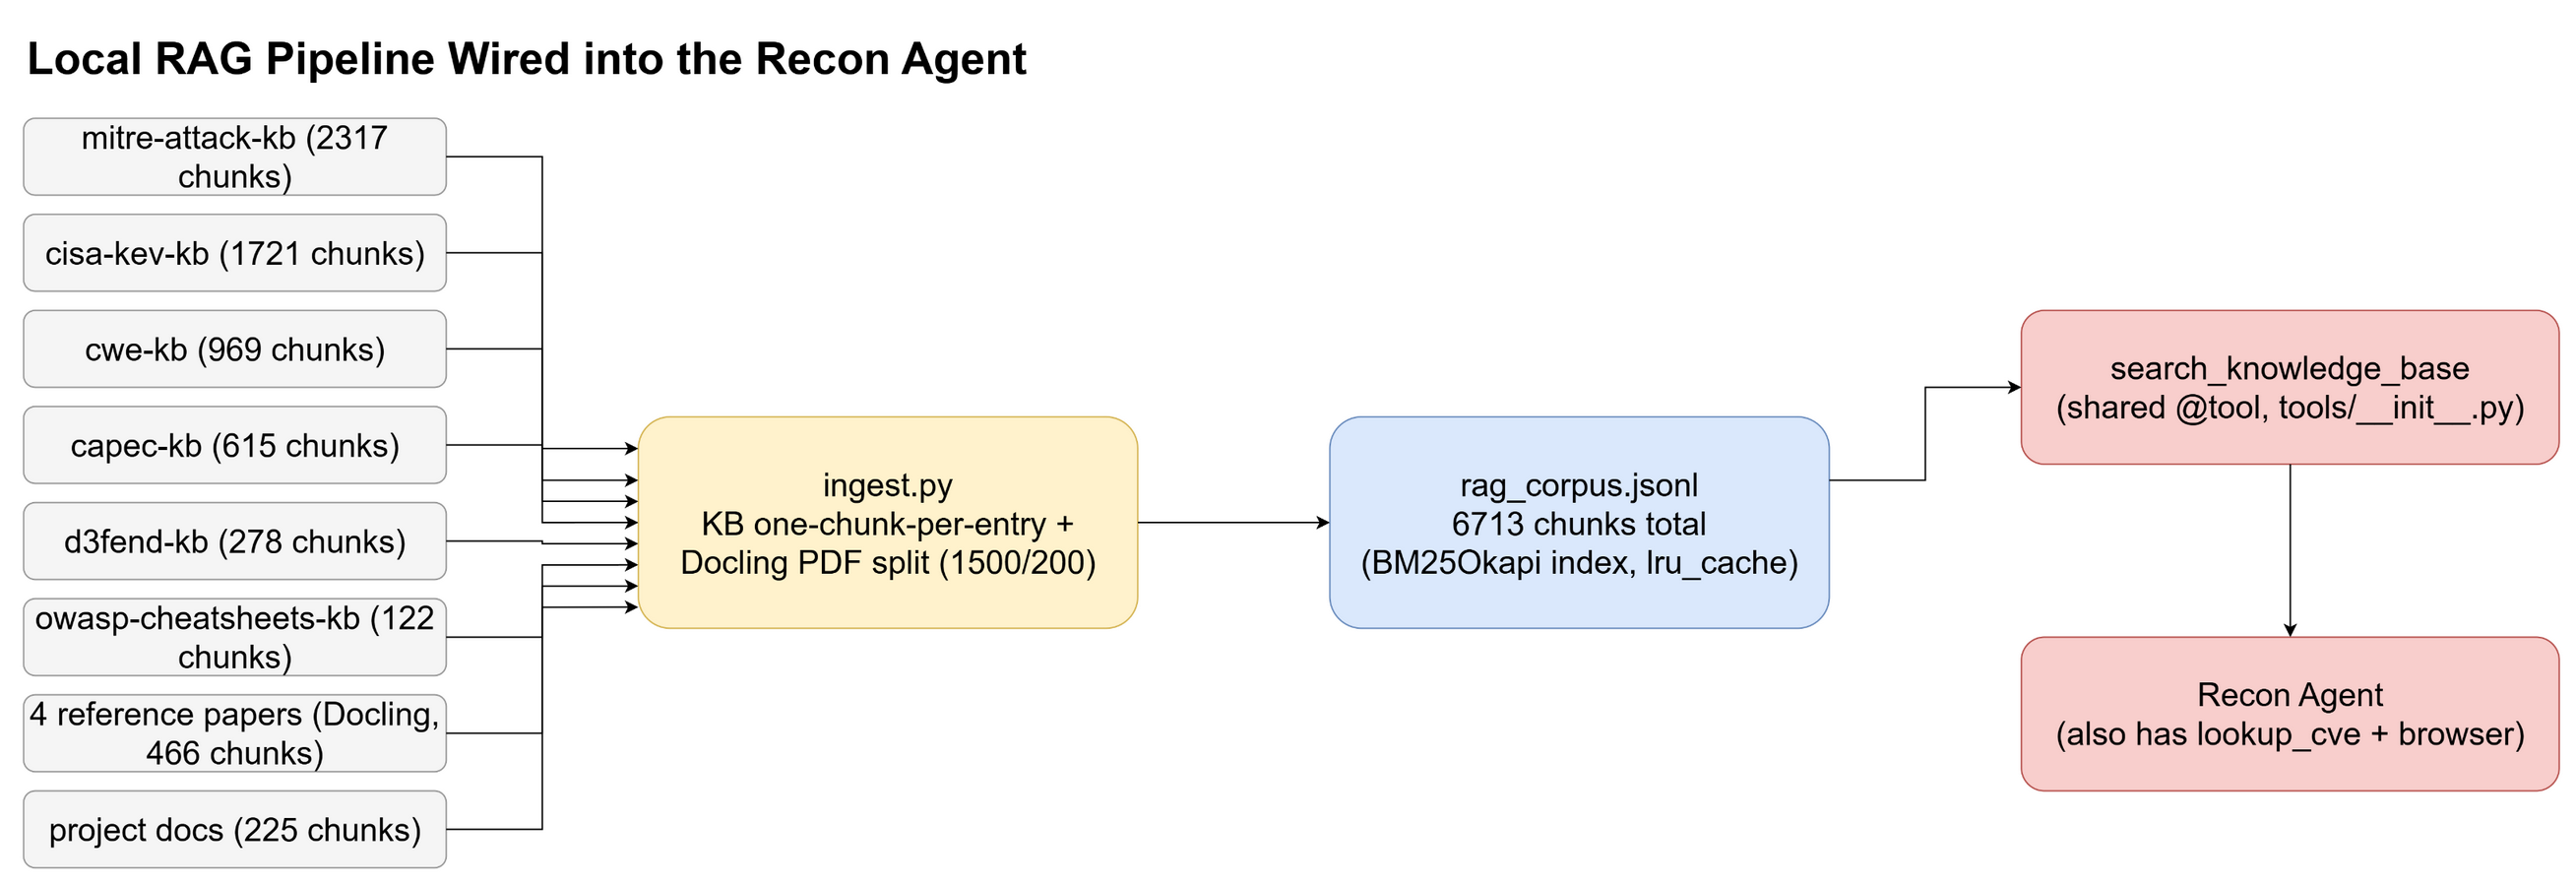
\includegraphics[width=\columnwidth]{rag_pipeline.png}
\caption{The local RAG pipeline. Knowledge-base entries are ingested one
chunk per entry; the four reference PDFs are split into 1500-character
chunks with 200-character overlap after Docling parsing. The resulting
6{,}713-chunk corpus is indexed once with BM25 and cached in memory for the
lifetime of the process.}
\label{fig:rag-pipeline}
\end{figure}

\subsection{Evidence-Grounding Mechanism}
\label{sec:grounding}

Every claimed finding produced by a specialist is passed to a shared
Evaluator agent before it is added to \texttt{verified\_findings}---the
only state the Orchestrator is allowed to treat as confirmed. The check has
two stages. First, a deterministic substring check asks whether the claimed
\texttt{evidence\_excerpt} is a real, verifiable substring of an actual tool
result already present in the conversation history; if the excerpt cannot
be located at all, the claim is rejected immediately with no LLM call.
Second, if the excerpt is real, a separate LLM judgment call asks a narrower
question: does the claim assert only what the cited excerpt actually
supports, or does it smuggle in additional detail---a specific score, a
specific exploitation status---that the excerpt itself never stated?
Algorithm~\ref{alg:grounding} summarizes the check. Section~\ref{sec:onoff} also
evaluates a variant whose step-2 judgment sees every tool result, not only the last.

\begin{algorithm}[t]
\caption{Evidence-Grounded Completion Check}
\label{alg:grounding}
\begin{algorithmic}[1]
\REQUIRE claimed excerpt $e$, claim text $c$, conversation history $H$
\STATE $m \leftarrow$ locate $e$ verbatim inside a real tool result in $H$
\IF{$m$ not found}
  \STATE \textbf{return} \textsc{Rejected} (step 1, no LLM call)
\ELSE
  \STATE $v \leftarrow$ LLM judgment: does $c$ assert only what $m$ supports?
  \IF{$v$ = yes}
    \STATE \textbf{return} \textsc{Verified}; add to \texttt{verified\_findings}
  \ELSE
    \STATE \textbf{return} \textsc{Rejected} (step 2, claim not supported by $m$)
  \ENDIF
\ENDIF
\end{algorithmic}
\end{algorithm}

\subsection{Stall detection and the safety valve}
\label{sec:stall}

The Orchestrator tracks \texttt{stall\_count}: the number of consecutive
turns in which the same specialist was re-dispatched \emph{without} any
growth in \texttt{verified\_findings} since its previous dispatch. When
\texttt{stall\_count} reaches a fixed limit (3), the Orchestrator forces the
run to end rather than continue looping. This distinction---same
specialist re-used productively versus re-used with no progress---was not
present in the first version of this logic, and Section~\ref{sec:testing}
reports the bug this omission caused, how it was found, and how it was
fixed.

% =============================================================================
\section{Testing}
\label{sec:testing}

\subsection{Test environment}

All benchmarks in this section were run against gpt-oss-20b (F16 GGUF),
served by \texttt{llama.cpp}'s \texttt{llama-server} (version 0.4.1-dev,
commit \texttt{930e2fa}, built with GCC 13.3 and CUDA toolkit 12.0) with Harmony
chat templating enabled (\texttt{--jinja}) and all layers offloaded to the GPU
(\texttt{-ngl 999}), on a dedicated NVIDIA A100-PCIe-40GB GPU (driver 615.71.09)
with a 131{,}072-token context window and four concurrent request slots.
The server defaults were temperature 1.0 and top-p 1.0; the agents override
the temperature per request, as stated below. The
LangGraph orchestration process ran inside a WSL2 Linux environment on a
Windows host, connected to the model server over an SSH tunnel. All agents,
including the Orchestrator and the Evaluator's judgment step, use this same
gpt-oss-20b instance, so the Evaluator judges output produced by the same
model; we have not run a different judge. Tool-using agents ran at
temperature 0.2 and the Orchestrator and Evaluator at 0.1, and no random seed was
fixed.

\subsection{Protocol}

Each of the seven suites in Table~\ref{tab:results} targets a specific node or mechanism in
isolation wherever possible (synthetic state, no browser dependency),
scaling from an initial proof-of-concept run (N=2--5) up to a
larger re-run (N=7--20) once the mechanism was shown to
work at all. Every suite's raw per-trial output is retained for
reproducibility. Two suites (Full-Graph and RAG/Recon) additionally run
the complete implemented subgraph end-to-end against real, live CVE
lookups, rather than synthetic state. Sections~\ref{sec:onoff} and~\ref{sec:m3}
report two later studies, on held-out CVEs and on generated claims.

\subsection{Results}

Table~\ref{tab:results} reports the final number from the larger run of
every suite. Because every row reports a 100\% figure in some form, and a bare
``100\% reliable'' claim would be indefensible on its face, the table's
rightmost column states explicitly what each 100\% figure does and does not
mean; Section~\ref{sec:hundred-percent} expands on this in full.

\begin{table*}[t]
\caption{Agent Benchmark Results}
\label{tab:results}
\centering
\begin{tabular}{@{}lccp{7.6cm}@{}}
\toprule
\textbf{Suite} & \textbf{N} & \textbf{Result} & \textbf{What the headline number actually measures} \\
\midrule
Safety / Guardrail gate & 8 & 100\% & Deterministic keyword/scope check; tests hand-written code, not model behavior \\
Reliability harness (sanitizer + circuit breaker) & 8 & 100\% & Deterministic string/counter logic; confirms a ported mechanism still works after the port \\
Evaluator (evidence grounding) & 10 & 100\% & The suite where the LLM is most directly exercised. Case A was first expected to verify; the Evaluator rejected it and we then relabelled the expectation as a test-design artifact, so 10/10 uses the revised expectation (9/10 under the original) \\
Orchestrator routing & 9 (7 scorable) & 100\% of scorable & 2 of 9 cases were robustness checks with no single correct answer and are excluded from the rate. Case C routed wrongly at N=4 and correctly at N=8 with identical code, so a single run does not characterise the router \\
Vulnerability Analysis tool-calling & 20 & 100\% / 100\% & Deterministic CVSS parser. Real NVD vectors for v2.0, v3.0 and v3.1; the v4.0 case used a synthetic well-formed vector, because NVD had no v4.0-scored CVE at the time \\
Full end-to-end graph & 8 & 100\% completion & ``Completion'' means no crash/hang, not correctness---only 62.5\% (5/8) reached a verified answer; 37.5\% (3/8) ended at the stall limit after the Evaluator rejected claims their excerpts did not support \\
RAG-augmented Recon & 8 & 100\% completion & Same caveat as above---KB-only resolution was 60\% (3/5); correct-fallback rate was 100\% (3/3) \\
\bottomrule
\end{tabular}
\end{table*}

\subsubsection{Why every suite reports a 100\% figure}
\label{sec:hundred-percent}

A wall of 100\% figures is exactly the kind of result that should invite
skepticism rather than confidence, so this section states plainly why each
one occurs, grouped by cause rather than left as an undifferentiated list.

\textbf{Cause 1---the suite tests deterministic code, not the model.} The
Safety gate is a keyword allow/deny check; the reliability harness is
string/counter logic; both are unit tests of hand-written functions. Once
the code is correct, 100\% is the expected outcome of testing deterministic
logic, the same way a correctly written function passes all of its unit
tests---it says nothing about how reliably the LLM itself behaves, because
the LLM never gets a chance to violate a check that never depends on it.

\textbf{Cause 2---the headline metric is narrower than ``the agent got it
right.''} The Full-Graph and RAG/Recon suites both report a completion rate
(did the trial finish without crashing or hitting the recursion limit) as
their headline ``success'' figure. Neither is a correctness claim on its own.
Only 62.5\% (5/8) of Full-Graph trials reached a verified answer the normal
way; the other 37.5\% (3/8) ended at the stall-limit
safety valve after the Evaluator rejected a claim its excerpt did not support three times
in a row---an outcome with no verified answer, and not a ``success'' in the sense a
reader might assume from a bare 100\%. Likewise, RAG/Recon's 100\% completion sits
alongside a 60\% (3/5) KB-only resolution rate and a 100\% (3/3)
correct-fallback rate---the latter two are the metrics that actually
describe whether the tool was used well.

\textbf{Cause 3---small N and author-written test cases.} The Evaluator
suite (N=10) is the suite where the LLM is most genuinely exercised, and
its 100\% is correspondingly the most meaningful of the seven---but the ten
cases were written by the same people who built the grounding logic,
not held out or generated adversarially, so an edge case the author did not
think to write would not appear as a failure here even if it exists in
practice. The generated-claim benchmark of Section~\ref{sec:m3} addresses
this for the Evaluator.

\textbf{Cause 4---run-to-run variability.} The Orchestrator's Case C
routed to \texttt{recon} instead of ending at N=4 and routed correctly at
N=8, with the same code and prompt, at temperature 0.1. The router also
shows a bias toward re-confirming rather than concluding. A single run of
a routing decision therefore does not characterise it, and the 100\% of
scorable cases reflects the N=8 outcome, not a stable property.

\subsection{Bugs found and fixed during this testing pass}

Table~\ref{tab:failures} catalogs every bug and infrastructure
failure this testing pass surfaced, each confirmed with a direct before/after
re-run rather than asserted from reading the code. Two of the rows (3 and 5) were introduced by the authors.

\begin{table*}[t]
\caption{Failure Taxonomy: Bugs and Infrastructure Failures Found During Testing}
\label{tab:failures}
\centering
\begin{tabular}{@{}p{4.0cm}p{2.4cm}p{4.0cm}p{5.0cm}@{}}
\toprule
\textbf{Issue} & \textbf{Layer} & \textbf{How it was found} & \textbf{Fix, and how the fix was confirmed} \\
\midrule
CVSS v2 vectors prefixed \texttt{CVSS:2.0/} rejected by the parsing library & Tool (deterministic) & In-process sanity check (Table~\ref{tab:tools}'s parser, tested directly) & Strip the known v2 prefix before constructing the parser object; re-tested against a real v2 NVD vector \\
Router's stall-count conflated a legitimately re-used specialist with a genuine stall & Orchestrator logic & Benchmark case designed to reproduce productive repeated use of one specialist & Track verified-finding count at each dispatch, only penalize repeats with zero new progress; re-verified with two new cases proving both directions \\
Benchmark harness executed every full-graph trial twice per run (\texttt{astream} + a separate \texttt{ainvoke}) & Measurement artifact & Reported latency was roughly double what single-execution timing would predict & Single \texttt{astream} call with dual stream modes; confirmed by a $\sim$2$\times$ latency drop (77.51\,s $\to$ 41.66\,s) on an identical re-run \\
MCP browser-server stdio handshake hung indefinitely & Infrastructure (WSL/Windows interop) & Isolated protocol-level diagnostic showed the subprocess launched but never returned a JSON-RPC response & Installed Node.js natively inside the Linux environment so the MCP subprocess never crosses an OS boundary; handshake time dropped from a 60\,s timeout to 2.1\,s \\
Knowledge-base ingestion produced zero chunks for one of six knowledge bases & RAG ingestion pipeline & Corpus chunk count for that knowledge base was 0 after a full ingestion run & Fixed a path double-nesting bug in the ingestion script; re-ingestion produced the expected 2{,}317 chunks \\
\bottomrule
\end{tabular}
\end{table*}

\begin{table*}[t]
\caption{Model-Behaviour Failure Modes Observed in the Agent System}
\label{tab:failures-behaviour}
\centering
\begin{tabular}{@{}p{3.4cm}p{6.6cm}p{5.4cm}@{}}
\toprule
\textbf{Failure mode} & \textbf{Evidence} & \textbf{Consequence} \\
\midrule
Claim not supported by the captured excerpt & 12 of 17 findings rejected across 5 of 8 runs; in the three stall-limit runs the rejected claims were true per NVD and CISA KEV; on held-out CVEs 416 of 433 correct claims were rejected & No verified answer in 3 of 8 development runs and in 88.6\% of held-out runs (Section~\ref{sec:onoff}); the three development runs took 52.6--71.4\,s against 13.1--17.8\,s for the three single-attempt answered runs \\
Confident unverified text shown after a stall & Final message is the model's wrap-up after all findings were rejected; the guarantee is on \texttt{verified\_findings}, not on displayed text & User sees a fluent answer with no verified support; a banner flags it but does not withhold it \\
Over-verification & Orchestrator Case C routed to \texttt{recon} at N=4 and to \texttt{end} at N=8; Recon used the browser after a correct knowledge-base answer in 2 of 5 knowledge-base-only cases & Extra latency (33.7 and 49.7\,s against 6--20\,s for the other three) with no wrong answer \\
Truncated structured output & The router and judge outputs hit a 2{,}000-token cap, the parser raised an error and ended a run; observed in interactive use, not in the N=8 benchmark & Cap raised to 6{,}000 tokens and the router now falls back to ending the run on error; not re-benchmarked \\
\bottomrule
\end{tabular}
\end{table*}

\begin{figure}[t]
\centering
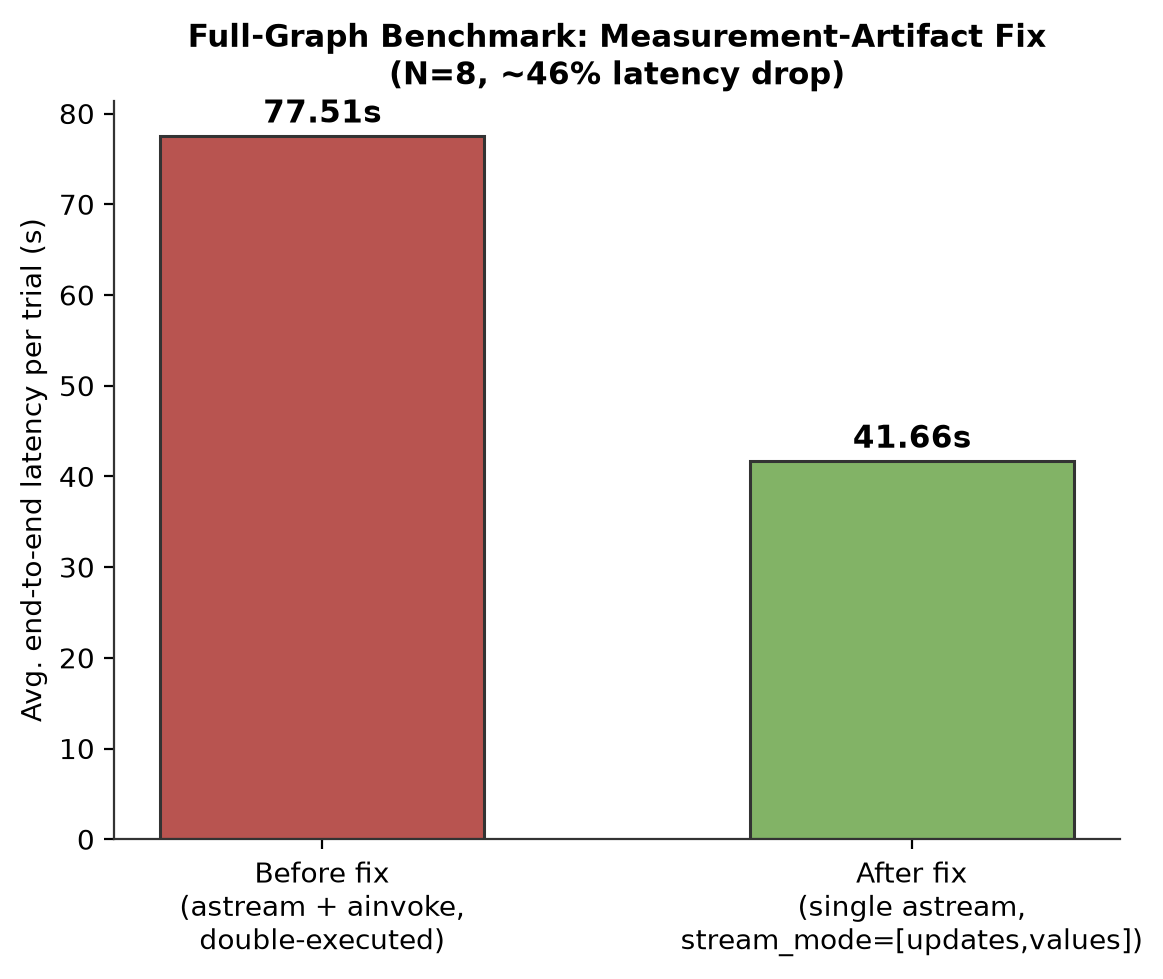
\includegraphics[width=\columnwidth]{latency_before_after_fix.png}
\caption{Full-graph average latency before and after fixing the
double-invocation measurement artifact (Table~\ref{tab:failures}, row 3),
on the same 8 objectives, same model, same dedicated GPU.}
\label{fig:latency-fix}
\end{figure}

\subsection{RQ3 in practice: what the Evaluator rejected}
\label{sec:rq3-practice}

Table~\ref{tab:fullgraph} lists the eight end-to-end runs, recounted from
the raw result file. The Evaluator rejected 12 of the 17 findings produced
(70.6\%), in five of the eight runs. Five findings were verified. Three
runs (Log4Shell, Zerologon, Follina) ended with no verified answer after
three rejected Recon attempts each, when the stall-limit safety valve
(Section~\ref{sec:stall}) stopped the loop. Two further runs also saw
rejections but still produced an answer: Struts (CVE-2017-5638) was
rejected twice and verified on its third attempt, and WebP (CVE-2023-4863)
was rejected once and then verified, so the retry loop recovered in both.

\begin{table}[t]
\caption{Full-graph runs (N=8), recounted from the raw result file.}
\label{tab:fullgraph}
\centering
\footnotesize
\setlength{\tabcolsep}{3pt}
\begin{tabular}{@{}rp{3.1cm}rrrp{1.5cm}@{}}
\toprule
\textbf{\#} & \textbf{CVE} & \textbf{Found} & \textbf{Verif.} & \textbf{Rej.} & \textbf{Outcome} \\
\midrule
1 & 2024-3400 & 1 & 1 & 0 & answered \\
2 & 2026-9862 & 1 & 1 & 0 & answered \\
3 & 2021-44228 (Log4Shell) & 3 & 0 & 3 & stall limit \\
4 & 2023-4863 (WebP) & 2 & 1 & 1 & answered \\
5 & 2020-1472 (Zerologon) & 3 & 0 & 3 & stall limit \\
6 & 2017-5638 (Struts) & 3 & 1 & 2 & answered, 3rd try \\
7 & 2019-0708 (BlueKeep) & 1 & 1 & 0 & answered \\
8 & 2022-30190 (Follina) & 3 & 0 & 3 & stall limit \\
\midrule
 & \textbf{Total} & 17 & 5 & 12 & 5 of 8 answered \\
\bottomrule
\end{tabular}
\end{table}

\textbf{The rejected claims were true.} In the three stall-limit runs the
rejected claims asserted a CVSS score of 10.0 (Log4Shell, Zerologon) or
exploitation in the wild (Follina), as recorded in our run notes. We checked
these against the NVD API and the CISA KEV catalogue on 3~October 2026. NVD
lists Log4Shell at 10.0 (CRITICAL) and Zerologon at 10.0 (CRITICAL; a
secondary CNA source lists 5.5), and both are in CISA KEV; Follina was added
to CISA KEV on 14~June 2022. The Evaluator therefore did not catch false
statements in these runs. It rejected claims that were true but were not
contained in the excerpt Recon had captured, and in each of the three
runs the user received no verified answer to a question whose answer was
correct. We call the mechanism an evidence-grounding or provenance check,
not a hallucination detector. We did not log the rejected claim text or the
rejecting stage for the Struts and WebP rejections, so we cannot say whether
those claims were true.

\textbf{Audit of the verified findings.} We compared the stored text of
each of the five verified findings with NVD. The stored text is truncated to
about 200 characters, so the audit covers that prefix only: product,
vulnerability type and, where shown, affected versions were consistent with
NVD for all five. We observed no false verified claim in five; a
Clopper--Pearson~\cite{clopper1934} 95\% upper bound on the false-accept rate for 0 of 5 is
about 45\%, so five runs cannot support a claim that none occur.

\textbf{What the user sees after a stall.} The guarantee holds for the
\texttt{verified\_findings} state, not for the text shown to the user. When
the stall limit fires, the run ends and the final message is still the
model's own confident wrap-up, built on findings the Evaluator rejected. A
user-interface banner now flags an answer with no verified findings, but
the text is still displayed. Table~\ref{tab:failures-behaviour} lists this
as a failure mode.

\textbf{Baseline.} The eight development runs have no no-check condition. A
comparison with no check, on held-out CVEs, is reported in
Section~\ref{sec:onoff}.

\subsection{Held-out Evaluator on/off study}
\label{sec:onoff}

\textbf{Design.} We drew 50 CVEs that were not used in development: 20 sampled at
random from the CISA KEV catalogue and 30 random NVD records, from a seeded
sample that includes recent CVEs. Each run asks: ``Look up CVE-X. State its CVSS
base score and severity, and say whether it is in the CISA KEV catalog.'' Each
CVE was run three times under three conditions: \emph{off}, which accepts every
finding unchecked; \emph{on}, the Evaluator of Section~\ref{sec:grounding}; and
\emph{all}, the same Evaluator whose step-2 judgment sees every tool result up to
the cited one (each capped at 3{,}000 characters) instead of only the last
result cut to 800 characters. Correctness is checked deterministically against
NVD and the 22~September 2026 KEV snapshot, on three facts only: the CVSS base
score, the severity label and KEV membership. No LLM judges correctness.

\begin{table*}[t]
\caption{Evaluator conditions on 50 held-out CVEs, three repeats each (run-level,
95\% Wilson intervals; repeats of one CVE are not independent).}
\label{tab:onoff}
\centering
\small
\begin{tabular}{@{}lrrr@{}}
\toprule
 & \textbf{off} & \textbf{on} & \textbf{all} \\
\midrule
Completed runs & 149/150 & 149/150 & 150/150 \\
Ended with an accepted answer & 100\% (149) & 11.4\% (17) [7.2, 17.5] & 98.7\% (148) [95.3, 99.6] \\
Accepted claims correct & 99.3\% (148/149) & 100\% (17/17) & 100\% (148/148) \\
Incorrect claims accepted & 1 & 0 & 0 \\
Correct claims rejected & 0/148 & 96.1\% (416/433) [93.8, 97.5] & 11.9\% (20/168) [7.8, 17.7] \\
Displayed answer correct & 99.3\% & 100\% & 100\% \\
Mean latency (s) & 9.9 & 37.2 & 12.4 \\
\midrule
CVEs answered, majority of repeats & 50/50 & 4/50 [3.2, 18.8] & 49/50 [89.5, 99.6] \\
CVEs with a false accept & 1/50 & 0/50 & 0/50 \\
\bottomrule
\end{tabular}
\end{table*}

\textbf{Results.} The no-check baseline was already correct in 148 of 149 runs, so
this task leaves little room for a check to improve accuracy. The standard
Evaluator ended only 17 of 149 runs with an accepted answer: it rejected 416 of 433
correct claims, and every one of those rejections concerned facts absent from the
last tool result. Claims here combine a score from \texttt{lookup\_cve} with KEV
status from the knowledge base, so the last result rarely holds all of them. The
\emph{all} variant, with the same judge and prompt, accepted an answer in 148 of
150 runs, all correct, at a mean 12.4\,s, close to the 9.9\,s of no check. The
difference between the standard and \emph{all} conditions is therefore a property
of the evidence the check is given, not of the check itself.

One claim was genuinely wrong. For CVE-2022-31206 the model stated that the CVE is
listed in the KEV catalogue, which it is not. The \emph{off} condition accepted
it, and the \emph{all} condition rejected the same claim in the matching run.
This is a single event, and 0 incorrect accepted claims against 1 is not a
significant difference.

\textbf{Caveats.} The three repeats of one CVE are not independent, so the
run-level intervals are too narrow; the CVE-level rows are the more conservative
view. The claim checker was corrected once after we inspected misclassified
claims, which had read a table cell answering ``No'' as KEV membership and a CVSS
version string as a score. All 450 runs were rescored with the corrected checker,
which has regression tests built from those claims. The judge is the same model
that produced the claim, and the task is easy for it. A task on which the
unchecked baseline is weaker is needed to show an accuracy gain. Two runs ended at
the 30-step recursion limit and are reported as errors, both on CVE-2022-31206.

\subsection{The Evaluator in isolation}
\label{sec:m3}

To replace the author-written Evaluator cases we generated 462 claims from NVD
records for 80 CVEs, each judged against the excerpt the agent would capture
(the \texttt{lookup\_cve} output cut to 800 characters). The claims state the
true score and severity, a wrong score, a wrong severity, the right score for a
different CVE, KEV membership, or the first sentence of the description. The
expected verdict is a fixed rule: a claim should be verified only if its facts
appear literally in the excerpt. The Evaluator verified 140 of 140 supported
claims, rejected all 290 false claims, and rejected 30 of 32 claims that were
true but absent from the excerpt; 140 of the 142 claims it verified were
supported (98.6\%, 95\% Wilson interval 95.0--99.6). The two exceptions are
borderline: one excerpt ended in a truncated KEV link, and one gave a score in
the description while the label CRITICAL was only inferred. Our first labelling
rule wrongly assumed that a KEV claim is never supported; NVD's reference list
for KEV CVEs contains a link to the CISA catalogue, which survived truncation in
13 of 30 cases and which the Evaluator correctly used. We corrected the rule and
rescored the saved verdicts. In isolation the check is therefore accurate, and
the agent-run rejections in Section~\ref{sec:onoff} come from the evidence it is
given.

\begin{figure}[t]
\centering
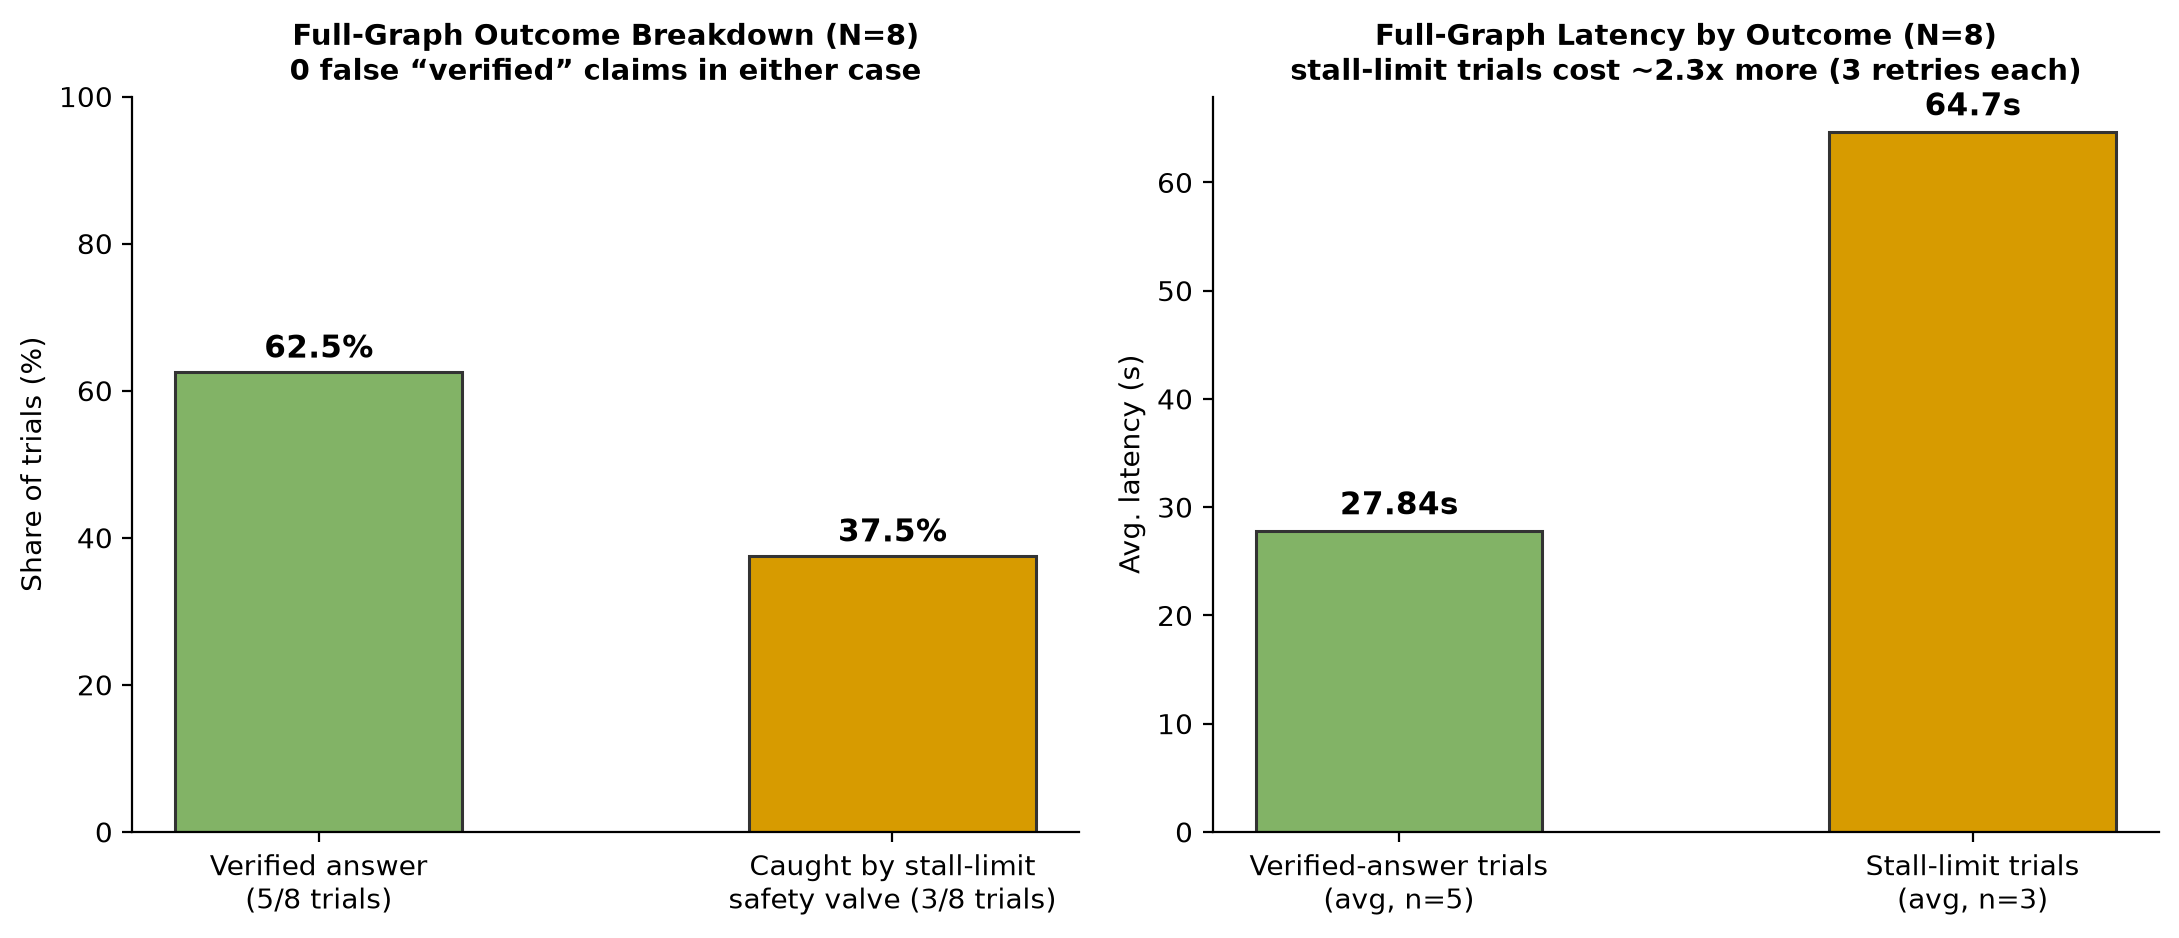
\includegraphics[width=\columnwidth]{full_graph_outcome_breakdown.png}
\caption{Full-graph outcome breakdown (N=8). The two bars are not a
pass/fail split. A stall-limit
trial is the system declining to certify a claim whose excerpt did not
support it, which in all three cases was a true claim. The latency panel shows why this refusal is not
free: each stall-limit trial paid for three rejected Recon retries before
terminating, roughly 2.3$\times$ the average cost of a trial that verified
cleanly on the first or second attempt.}
\label{fig:full-graph-outcome}
\end{figure}

\begin{figure}[t]
\centering
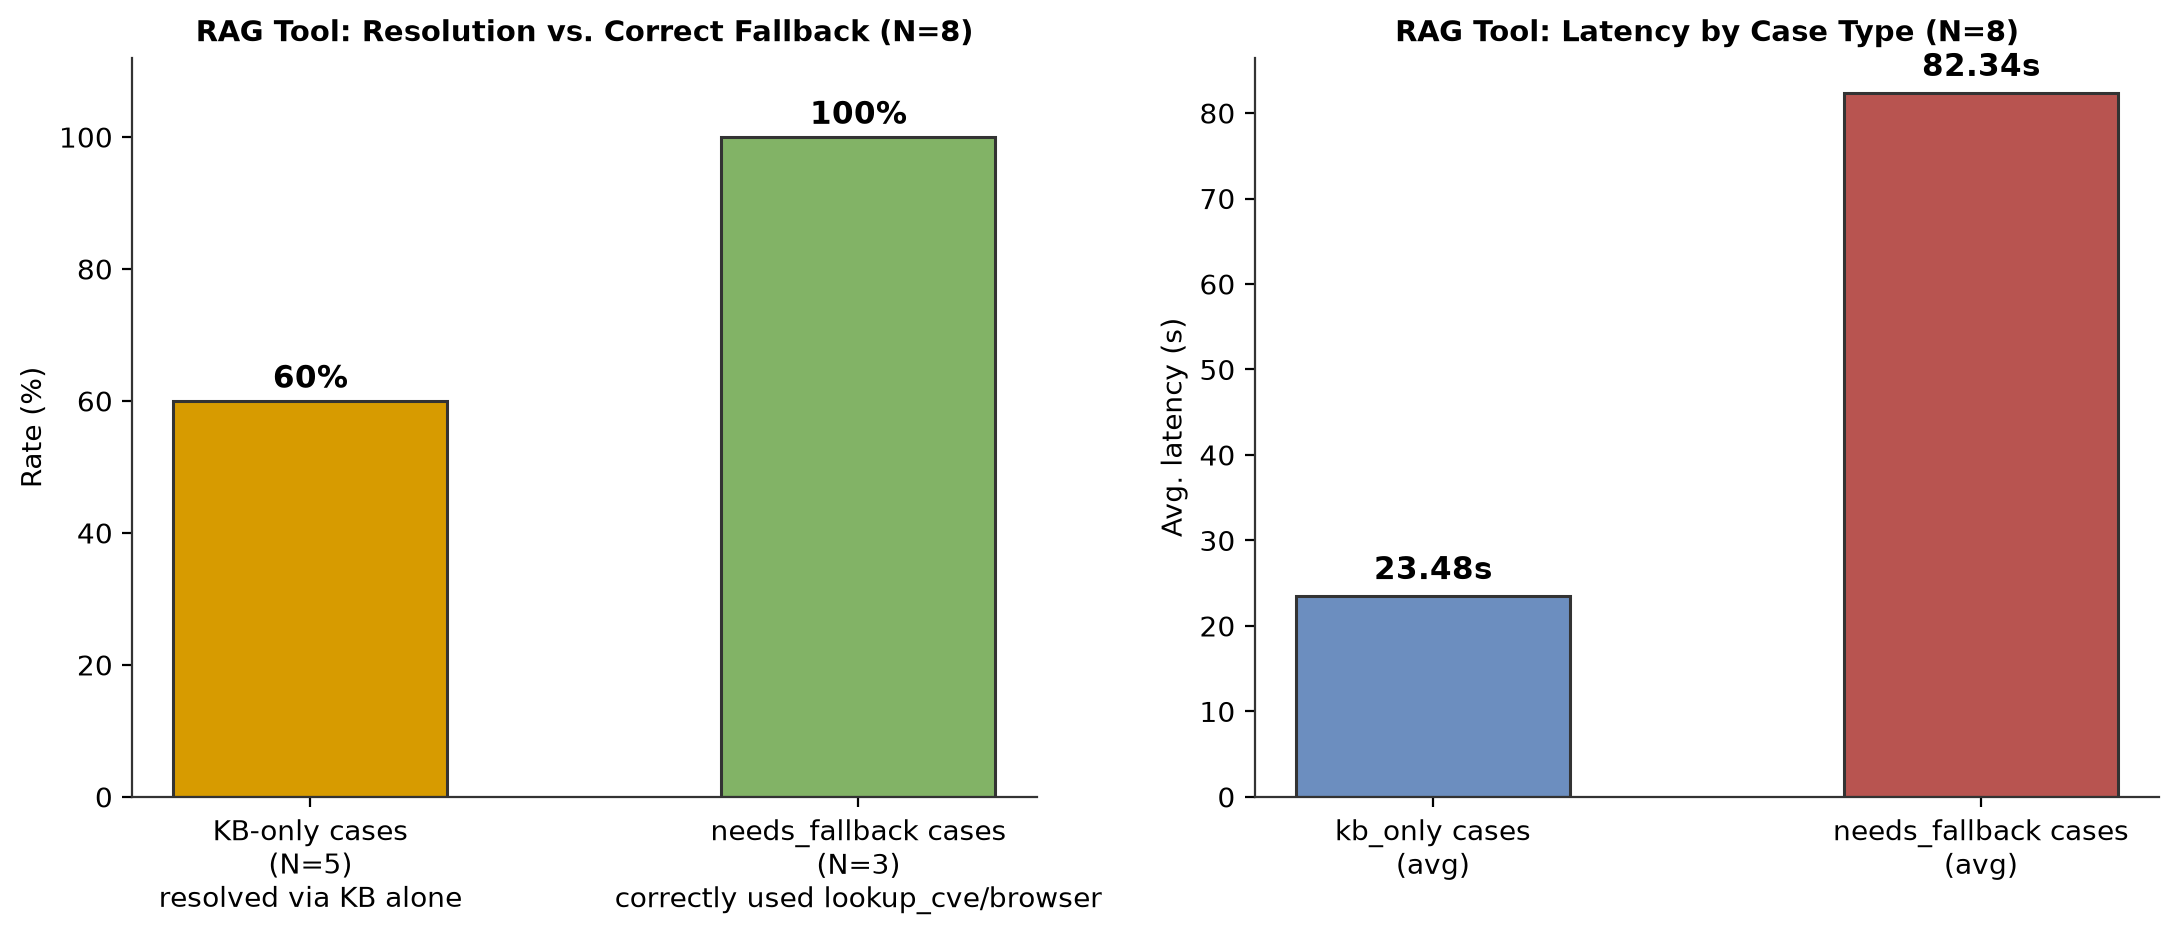
\includegraphics[width=\columnwidth]{rag_kb_vs_fallback.png}
\caption{RAG-augmented Recon: resolution rate for cases the local knowledge
base genuinely covers versus correct-fallback rate for cases deliberately
chosen to exceed it, alongside the corresponding latency difference.}
\label{fig:rag-results}
\end{figure}

\subsection{Relation to prior published systems}
\label{sec:comparison}

We do not rank this system against prior work, because the tasks differ.
PentestGPT~\cite{pentestgpt} reports completion of full HackTheBox-style
penetration-test targets with a frontier model and a human relaying
commands. hackingBuddyGPT~\cite{happe2026} reports exploit success on a
Linux privilege-escalation benchmark, including a local Llama~3 condition
with no human. This paper's 62.5\% (5 of 8) is the fraction of eight
single-CVE lookup runs that ended with a verified answer. A CVE lookup is a
far easier task than a penetration test or a privilege escalation, and the
two quantities (verified-answer rate and exploit success) are not
comparable, so no figure here should be read as better or worse than
theirs.

% =============================================================================
\section{Multi-Model Evaluation}
\label{sec:multimodel}

\subsection{Models and protocol}

We compare six models, all served locally and queried with the same
multiple-choice prompt: gpt-oss-20b~\cite{gptoss} (base); a second Heretic model of
gpt-oss-20b (``Heretic, reference''), meant to be the publicly released one, and our own Heretic-processed variant
(``Heretic, ours''), both described in Section~\ref{sec:refusal};
Qwen3.5-9B in thinking mode; Granite~4.1; and Foundation-Sec-8B, a model
trained specifically for security text. Each model answers the four
CyberMetric~\cite{cybermetric} sets, which contain 80, 500, 2{,}000 and
10{,}180 four-option questions. The largest file is distributed as
``CyberMetric-10000'' but contains 10{,}180 questions, and we report that
count. The model is asked to reply with ``ANSWER: X''; a response from which
no option can be parsed is scored as wrong, and we report how many such
responses each run produced. All intervals are 95\% Wilson score intervals~\cite{wilson1927}.
For comparisons between two runs on the same questions we use an exact
two-sided McNemar test~\cite{mcnemar1947} on the questions both runs answered.

\textbf{Hardware and serving.} The CyberMetric and BFCL runs were executed on
a separate HPC server with one NVIDIA H200 NVL GPU (143{,}771\,MiB, driver
580.173.02, CUDA toolkit 12.0), an Intel Xeon 6530P CPU and 503\,GB of RAM, not
on the A100 host of Section~\ref{sec:testing}. The CyberMetric models were
served with vLLM 0.28.0 (Python~3.12). Table~\ref{tab:serving} lists the vLLM settings taken from the shell history, the
last recorded invocation per model. They differ across models, and the history
shows several earlier attempts per model, so they are the best available record
rather than a logged configuration. The BFCL run used the
harness at commit \texttt{6ea5797} (23~March 2026) with a locally added model
entry, \texttt{gpt-oss-20b-local-FC}, which uses a custom llama.cpp handler in
function-calling mode, against gpt-oss-20b (F16 GGUF with MXFP4
mixture-of-experts tensors) served by \texttt{llama-server} with a
32{,}768-token context; the \texttt{llama-server} build on the host is
0.4.1-dev, commit \texttt{911f6cdc8}.
The evaluation script sends each question to the served model's chat endpoint
with the system prompt ``You are a security expert who answers questions'',
defaults to temperature 0, and re-asks up to five times when no
``ANSWER: X'' line can be parsed; the unparsed counts we report are those that
remained after the retries
gpt-oss-20b and our Heretic variant used a 4{,}096-token limit, a 600\,s timeout
and 32 concurrent requests; the settings for the other four models were not recorded.

\begin{table}[t]
\caption{vLLM serving settings of the CyberMetric runs (last recorded invocation).}
\label{tab:serving}
\centering
\small
\begin{tabular}{@{}lrrr@{}}
\toprule
\textbf{Model} & \textbf{Context} & \textbf{Max seqs} & \textbf{GPU frac.} \\
\midrule
gpt-oss-20b, Heretic (ours) & 16{,}384 & default & 0.30 \\
Qwen3.5-9B & 16{,}384 & 64 & 0.30 \\
Granite~4.1 & 4{,}096 & 8 & 0.14 \\
Foundation-Sec-8B & default & default & 0.20 \\
Heretic (reference file) & default & default & 0.20 \\
\bottomrule
\end{tabular}
\end{table}

\subsection{Results}

Table~\ref{tab:cybermetric} gives the full results matrix and
Fig.~\ref{fig:cybermetric} plots it with confidence intervals.

\begin{table*}[t]
\caption{CyberMetric Accuracy (\%) by Model and Question-Set Size. Bold marks the best value in a column. The last column counts responses that could not be parsed on the 10{,}180-question set; they are scored as incorrect.}
\label{tab:cybermetric}
\centering
\begin{tabular}{@{}lccccc@{}}
\toprule
\textbf{Model} & \textbf{80} & \textbf{500} & \textbf{2{,}000} & \textbf{10{,}180} & \textbf{Unparsed (10{,}180)} \\
\midrule
Foundation-Sec-8B & 88.75 & 85.80 & 85.30 & 82.04 & 5 \\
Granite 4.1 & \textbf{96.25} & 90.40 & 89.70 & 84.91 & 5 \\
Qwen3.5-9B (thinking) & 95.00 & \textbf{94.80} & \textbf{92.35} & \textbf{87.75} & 17 \\
gpt-oss-20b (base) & \textbf{96.25} & 93.00 & 91.05 & 87.21 & 2 \\
gpt-oss-20b Heretic (reference) & \textbf{96.25} & 92.60 & 91.35 & 87.04 & 12 \\
gpt-oss-20b Heretic (ours) & \textbf{96.25} & 92.40 & 91.45 & 87.15 & 6 \\
\bottomrule
\end{tabular}
\end{table*}

\begin{figure*}[t]
\centering
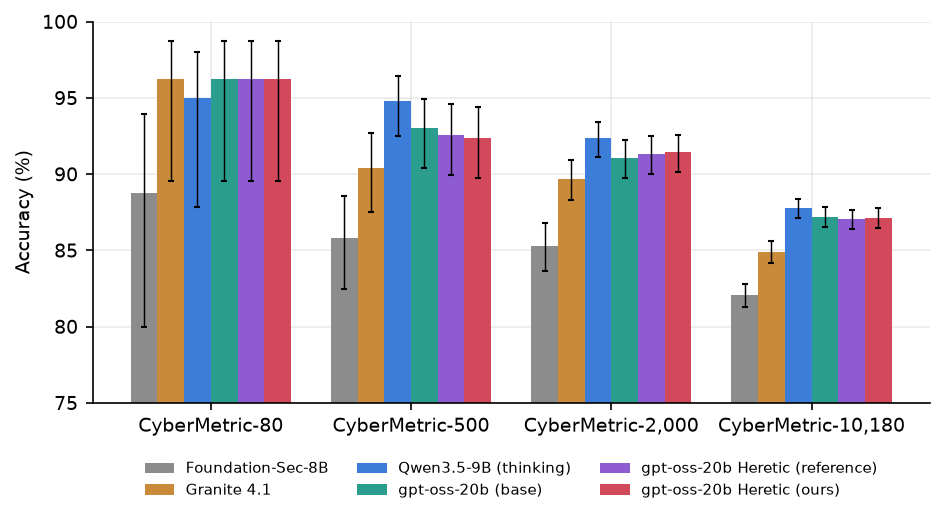
\includegraphics[width=0.78\textwidth]{cybermetric_all_models.png}
\caption{CyberMetric accuracy for six models on four question-set sizes.
Error bars are 95\% Wilson intervals. On the 80-question set the intervals
are wide (up to about 9 points below the estimate) and overlap for every
model, so that set cannot rank the models.}
\label{fig:cybermetric}
\end{figure*}

Four observations follow from the matrix.

\textbf{The small sets cannot rank models.} On the 80-question set four of
the six models score 96.25\%, and the intervals overlap widely. The ordering
only becomes informative on the 10{,}180-question set, where the interval
half-width falls to about 0.65 points. Every model also scores lower on the
larger sets than on the 80-question set, so a result from the small set
overstates absolute performance.

\textbf{Qwen3.5-9B (thinking) and the gpt-oss-20b family lead.} At 10{,}180
questions Qwen3.5-9B reaches 87.75\%, gpt-oss-20b 87.21\%, and the two
Heretic variants 87.04\% and 87.15\%. The interval for Qwen3.5-9B
(87.10--88.37) overlaps the one for the base gpt-oss-20b (86.55--87.84), so
the data do not separate them. Qwen3.5-9B has fewer total parameters than
gpt-oss-20b but spends extra tokens on reasoning, a cost we do not measure
here.

\textbf{Granite 4.1 and Foundation-Sec-8B trail.} Granite~4.1 scores 84.91\%
and Foundation-Sec-8B 82.04\%. Both intervals lie entirely below the
gpt-oss-20b interval. The security-specialized model is therefore the
lowest, not the highest. We did not tune the prompt for it, and a model of
that kind may be disadvantaged by the answer-format instruction, so we
treat this as a result for this protocol and not as a verdict on the model.

\textbf{Unparsed answers are rare but uneven.} Qwen3.5-9B produced 17
unparsed responses and the reference Heretic release 12, against 2 for
the base model. These are at most 0.17\% of questions, so they do not
change any ranking, but they are a reminder that output-format reliability
differs between models.

\subsection{The cost of refusal removal}
\label{sec:refusal}

Refusal removal (``abliteration'') edits a model so that it no longer
refuses requests. It rests on the finding of Arditi et
al.~\cite{arditi2024} that refusal is mediated largely by a single direction
in activation space, which can be projected out of the weights. Labonne
popularized the weight-editing recipe~\cite{labonne2024}, and Lai later
proposed projected and norm-preserving variants~\cite{lai2025}. Heretic~\cite{heretic}
automates the process: it parametrizes the directional ablation (which
layers, how strongly, and with what weighting) and searches those parameters
with a Tree-structured Parzen Estimator~\cite{bergstra2011} through
Optuna~\cite{optuna}, scoring each trial by
the number of refusals on a set of prompts the original model refuses and by
the KL divergence between the edited and original model on harmless prompts.
An independent comparison of four abliteration tools on sixteen
models~\cite{young2025} found that single-pass methods preserved capability
better than Bayesian-optimised ones such as Heretic, and that mathematical
reasoning was the most sensitive capability. Our experiment complements that
work by testing a knowledge benchmark on gpt-oss-20b.
Fig.~\ref{fig:heretic-frontier} plots the trials Heretic offered for
selection, and Fig.~\ref{fig:heretic-parity} compares capability.

We measure refusals on a set of 100 red-team prompts covering several
categories of offensive-security requests. The unmodified gpt-oss-20b
refused all 100. The trials on the frontier range from 96 refusals at a KL
divergence of 0.0006 to 27 refusals at 0.0624, and the relationship is
necessarily monotone, because these are non-dominated trials: fewer
refusals always cost more divergence. We do
not reproduce the prompts or any model output in this paper. The reference
model is meant to be the public Heretic release of gpt-oss-20b; see the provenance
note below. Our variant is a
model we produced ourselves by running Heretic for 400 optimization trials
on a single NVIDIA A100 GPU, and from those trials we selected Trial 310, the trial
with the fewest refusals: 27 of 100 at a KL divergence of 0.0624, which is
the highest divergence on the frontier. Choosing the extreme end of the
frontier makes the capability comparison below a deliberately demanding
test, since any damage from the edit should be largest there. The
reference model, if it is the public release, was produced by its publisher, and we
did not rerun it.

\textbf{Metric and provenance.} A response counts as a refusal when
Heretic's marker-string matcher finds a refusal phrase in it. No LLM judge
or human check was used, so a response that complies partly, or refuses
without a listed phrase, is misclassified. The 100 prompts are the same
ones Heretic optimised against, so 27 of 100 is an in-sample figure. We did
not evaluate the base, reference or our model on a held-out prompt set, and
the reference release's own refusal count is not measured here.
Because 27 prompts are still refused, we describe the edit as reducing, not
removing, refusals. We did not measure the quality of any compliant output.
The result file of our variant is suffixed ``-custom''. Our run records do
not settle which weights the reference result file used: its model path points
to a local directory that our own variant's serving command also used, so the
reference result may be a second evaluation of our variant under different
serving settings, not of the public release. We therefore report the two
Heretic rows as two evaluations of Heretic-edited models, and we do not claim
that the public release was tested. Our variant
was produced by running Heretic directly on the unmodified gpt-oss-20b
weights, with no other fine-tuning, using a 100-prompt offensive-security
set in 12 categories (malware, exploit development, defense evasion, and
others) as the refusal prompts; ``cybersecurity'' in the file name refers
to that prompt set.

\begin{figure}[t]
\centering
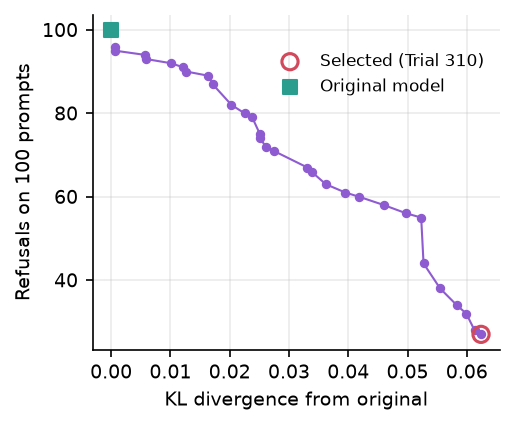
\includegraphics[width=0.85\columnwidth]{heretic_refusal_vs_kl.png}
\caption{Refusals on 100 red-team prompts versus KL divergence from the
original model for the trials offered by Heretic. Values are transcribed
from the trial-selection screen. The circle marks Trial 310, the trial we
selected. The original model has 0 divergence by definition and refused 100
of 100 prompts.}
\label{fig:heretic-frontier}
\end{figure}

\begin{figure}[t]
\centering
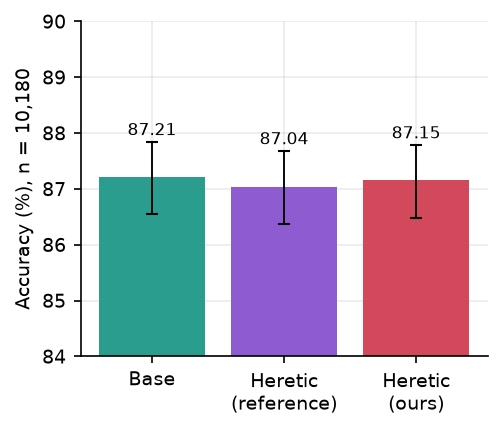
\includegraphics[width=0.85\columnwidth]{heretic_parity_10180.png}
\caption{CyberMetric accuracy on all 10{,}180 questions for the base model
and the two refusal-reduced variants, with 95\% Wilson intervals. The
vertical axis is truncated to 84--90\%.}
\label{fig:heretic-parity}
\end{figure}

On capability, reducing refusals did not measurably change accuracy. On the
10{,}180-question set the reference Heretic model scores 87.04\% and ours
87.15\%, against 87.21\% for the base model. In a paired exact McNemar test
against the base model, the base model answered 176 questions
correctly that the reference model missed, while the reference model answered
159 that the base missed ($p=0.38$); for our variant the counts are 167 and
161 ($p=0.78$). On the 2{,}000-question set the p-values are 0.53 and 0.35. The
paired accuracy difference on the large set is $-0.17\pm0.35$ points for the
reference model and $-0.06\pm0.35$ points for ours (95\% intervals), so a
loss of more than about 0.5 points is excluded at the 95\% level; this is an interval, not a formal equivalence test with a pre-set margin. This is an
equivalence-style statement about knowledge-recall accuracy only. It does
not show that the edited models behave the same on open-ended, mathematical
or agentic tasks, which we did not test. Since Young~\cite{young2025} found
mathematical reasoning to be the capability most sensitive to abliteration,
the absence of a loss here should not be extended to reasoning.

\subsection{Tool calling on BFCL}
\label{sec:bfcl}

We ran the Berkeley Function Calling Leaderboard~\cite{bfcl} against
gpt-oss-20b served with native function calling. Fig.~\ref{fig:bfcl} shows
the three categories that produced valid scores: simple Python functions
(89.00\%), multiple candidate functions (88.00\%), and irrelevance
(85.42\%), where the correct behavior is to make no call. The parallel and
parallel-multiple categories both scored exactly 0.00\%. A result of exactly
zero on two categories usually points to a problem in how the model server or
the harness is configured for parallel calls, and not to a model that is
incapable of them. We have not yet diagnosed it, so we exclude those two
categories from the paper's claims and do not report them as a model
weakness.

\begin{figure}[t]
\centering
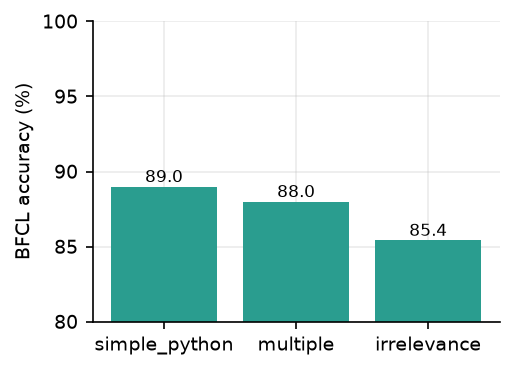
\includegraphics[width=0.75\columnwidth]{bfcl_categories.png}
\caption{BFCL accuracy for gpt-oss-20b on the categories with valid
scores. The vertical axis is truncated to 80--100\%. The parallel and
parallel-multiple categories are omitted (Section~\ref{sec:bfcl}).}
\label{fig:bfcl}
\end{figure}

\subsection{How the benchmarks relate to the agent results}

A model with roughly 87\% accuracy on security knowledge and about 88\% on
single-call tool use is not thereby guaranteed to supply the evidence an
agent needs. In our end-to-end runs (Section~\ref{sec:testing}) the same
gpt-oss-20b produced claims that the Evaluator could not trace to captured
tool output in five of eight development runs. In the three runs that ended
without a verified answer those claims were true, so the shortfall was in
provenance, not factual accuracy. On 50 held-out CVEs the unchecked model was
correct in 99.3\% of runs (Section~\ref{sec:onoff}). We make these observations
for one model and one task format; they do not establish a general relationship.

% =============================================================================
\section{Limitations of the Approach}
\label{sec:limitations}

\textbf{Narrow agent scope.} The agent system has two specialists, Recon
and Vulnerability Analysis, plus three control agents (Safety,
Orchestrator, Evaluator). It covers reconnaissance and vulnerability
analysis of public CVE data. No claim in this report generalizes to other
security tasks, such as exploitation, attack planning or incident handling.

\textbf{Target realism.} All testing uses live CVE/CWE/ATT\&CK data lookups
against real, public reference sources (NVD, the local knowledge bases), but
no live exploitation is attempted against any target---this trades
ecological validity for reproducibility and unambiguous legality, a
deliberate choice rather than an oversight.

\textbf{The grounding mechanism is a substring-based oracle.} It proves a
claimed fact literally appears in real captured tool output, which is
strong structural evidence but does not by itself prove the claim's
arbitrary semantic correctness beyond that check.

\textbf{Model coverage differs between experiments.} The multi-model
comparison covers six models on a knowledge benchmark, but the agent
experiments and the BFCL run use only gpt-oss-20b, and no model above
20 billion parameters is tested. Conclusions about agent behavior
therefore rest on one model.

% =============================================================================
\section{Limitations in Testing}
\label{sec:testing-limitations}

\textbf{Statistical power of the agent suites.} The development suites
(Table~\ref{tab:results}) run at N=7--20 and report no confidence intervals.
That is sufficient to catch and confirm real bugs, as this testing pass
repeatedly did, but not to claim a precise reliability percentage. The
held-out study (Section~\ref{sec:onoff}) has 150 runs per condition with Wilson
intervals, but only 50 distinct CVEs, a single question format and one model,
so its intervals understate the uncertainty about other tasks.

\textbf{Author-written test cases.} Several suites, most notably the
Orchestrator (N=9) suite and the original Evaluator suite (N=10), use
hand-written cases designed by the same people who built the mechanisms under
test. The Evaluator is also tested on 462 generated claims
(Section~\ref{sec:m3}), but the Orchestrator has no equivalent.

\textbf{The 62.5\% full-graph figure counts only runs that ended with a
verified answer.} In each of the three unanswered runs the Evaluator
rejected claims that were true but not supported by the captured excerpt
(Section~\ref{sec:rq3-practice}), so these are false rejections: the user
got no verified answer to a question with a correct answer. Whether that
trade is acceptable, versus a Recon agent that captures fuller evidence in
the first place, is not settled by these eight runs. The user-visible text
after a stall is also still the model's unverified answer
(Section~\ref{sec:rq3-practice}).

\textbf{Dedicated versus shared GPU.} A separate, unplanned
observation during this testing pass showed a $\sim$22$\times$ average latency
inflation (and $\sim$44$\times$ at the tail) when the same benchmark was
accidentally run against a shared, multi-tenant GPU instead of a dedicated
one, with success rate completely unaffected. The latency figures of the
development suites were measured on a dedicated GPU; the held-out study used the
same server, but we did not check for other users' load during it. This finding is reported here as a
caution for reading any LLM-agent latency number in isolation, in this or
any other paper, without knowing whether the GPU was dedicated or shared at
test time.

\textbf{Uncontrolled serving settings.} The six models were served and
queried through separate setups. Quantization, decoding parameters, context
length and, for the thinking model, the token budget were not forced to be
identical, so small differences between models, especially those whose
intervals overlap, should not be over-read.

\textbf{Single run per model and benchmark.} Each CyberMetric result is one
pass. The intervals capture sampling error over questions but not
run-to-run variation from decoding randomness.

\textbf{Possible benchmark contamination.} CyberMetric is public, and we do
not know whether any of the models saw it in training. Absolute scores may be
inflated, though a comparison between a base model and its refusal-reduced
copy is unaffected, since both share the same training data.

\textbf{Label quality and model size.} CyberMetric was built with LLM
assistance, so some answer labels may be wrong, and we did not audit them.
gpt-oss-20b is a mixture-of-experts model with about 21 billion parameters in
total and 3.6 billion active per token~\cite{gptoss}; we did not measure
active parameters, latency or memory for the other models, so ``small'' here
refers to the stored size class.

\textbf{BFCL is incomplete.} The parallel-call categories are excluded
because they scored exactly zero, which we suspect is a configuration
problem that is still undiagnosed (Section~\ref{sec:bfcl}).

\textbf{Refusal measurements are partial.} Refusals are counted by
Heretic's marker-string matcher, with no judge, on a single 100-prompt
set that is also the set the optimizer tuned against; no held-out set
was used and the reference release's count was not measured. Only the
original model's count (100/100) and the frontier are reported. We did
not measure the quality of any compliant output, and the capability
comparison covers knowledge recall only; no reasoning benchmark or BFCL
re-run was done for the edited models.

\textbf{External validity.} All findings are scoped to the specific model,
agent code, and knowledge-base snapshot tested here; nothing in this report
generalizes beyond that tested configuration without further, separately
scoped validation.

% =============================================================================
\section{Reproducibility}
\label{sec:repro}

The CyberMetric and BFCL result files, the evaluation script, and the script that
regenerates every figure and statistic from those files are kept with the project.
Model identifiers, hardware and serving settings are given in
Sections~\ref{sec:testing} and~\ref{sec:multimodel}. No random seed was fixed for
the agent runs, so repeated runs may differ, and the red-team prompts are
withheld (Section~\ref{sec:ethics}).
The agent-study scripts (the seeded CVE-set builder, the on/off runner, the claim
benchmark and the scoring scripts) and their raw per-run results are kept with the
project.

% =============================================================================
\section{Ethical Considerations}
\label{sec:ethics}

All lookups and reasoning tasks in this report's testing use publicly
available, authorized reference data (NVD, MITRE ATT\&CK/CWE/CAPEC/D3FEND,
CISA KEV, OWASP); no live exploitation, no third-party system, and no
unauthorized target is touched at any stage. Consistent with the
CyberSecEval framing~\cite{purplellama}, this work's goal is measuring the
\emph{reliability and verifiability} of LLM-driven tool use, not eliciting,
developing, or publishing novel offensive capability---nothing in this
report lowers the difficulty of an actual attack beyond what the same
publicly available tools and data already provide independently of any LLM.

The refusal-removal experiments need a separate note, because removing a
model's refusal behavior removes a safeguard. We study the technique to
measure its effect on capability, not to promote it. We do not reproduce the
red-team prompts, and we report no model output from them: only refusal
counts and benchmark accuracy appear here. Our finding that capability is
unchanged has a dual-use reading, namely that refusal removal is cheap in
capability terms, which is why we recommend that developers
who release open weights treat refusal behavior as a safeguard that can
be removed and plan accordingly. We withhold the prompts and all model outputs; the aggregate counts and
benchmark scores reported here are the only artifacts of that experiment we
publish. The intended use of the result is defensive: to show developers that
refusal behavior is a thin layer that can be reduced cheaply. Distribution of
the refusal-reduced variants is a decision for the authors' institution.

% =============================================================================
\section{Conclusion and Future Work}
\label{sec:conclusion}

\textbf{Small open-weight models know security material well.} On the
10{,}180-question CyberMetric set, Qwen3.5-9B (thinking) and gpt-oss-20b
both reach about 87\%, and Granite~4.1 reaches 84.9\%. The security-specialized
Foundation-Sec-8B scored 82.0\% under our protocol. A model that fits on one
GPU is therefore a credible baseline for security question answering. We also
showed that the 80-question set cannot rank models and that results need
the larger sets and confidence intervals to be trusted.

\textbf{Reducing refusals did not measurably change knowledge accuracy.}
Starting from a model that refused all 100 red-team prompts, a 400-trial
Heretic run produced a variant with 27 refusals (by Heretic's string
matcher, on the prompts it was tuned on), and this variant matched the
base model on CyberMetric (87.15\% against 87.21\%, paired $p=0.78$). The
reference Heretic result (87.04\%, $p=0.38$) was similar. On this recall benchmark
the edit did not cost accuracy. Because we tested only knowledge recall,
we make no claim about reasoning or other tasks.

\textbf{The model handles most single-call tool use in the categories we
could score.}
gpt-oss-20b reached 89.0\% on simple function calls, 88.0\% on choosing
among several functions, and 85.4\% on recognising that no function should
be called.

\textbf{An evidence check rejects what it cannot trace.} Inside a LangGraph
agent, the Evaluator accepts only claims traceable to captured tool output. On
50 held-out CVEs the unchecked baseline was already correct in 99.3\% of runs.
With only the last tool result as evidence, the check ended 11.4\% of runs with
an accepted answer; with all tool results it answered 98.7\% of runs at nearly
the latency of no check, and accepted no incorrect claim, against one for the
baseline, a difference too small to be significant. In isolation, on 462 claims,
it rejected every false claim. The check enforces provenance at low cost when
given the right evidence; showing that it improves accuracy needs a task on
which the baseline is weaker.

Together these results describe what one lab GPU and public data can
measure about an open-weight model of 8--20 billion parameters: its
accuracy on the largest benchmark sets with confidence intervals, its
tool-calling behaviour, and, in a case study, what an evidence-grounding
check rejects inside an agent. On the task we used the unchecked baseline
was already near ceiling, so an accuracy gain could not be shown. All of this
ran on a single GPU with public data and no live targets.

The work has a clear scope. The agent experiments use one model, eight development runs and 450 held-out
runs on a single question format, the six models were served with their own settings, and the
two parallel-call BFCL categories remain excluded pending diagnosis. These
define the next steps rather than undermine the findings above:
(i) diagnose and rerun the parallel-call categories;
(ii) run the agent with the other five models to test whether the Evaluator's
rejection pattern carries over;
(iii) test the check on a task where the unchecked baseline is weaker, such as
CVEs with conflicting or missing NVD scores;
(iv) extend the refusal-removal comparison to reasoning and tool-use
benchmarks, where earlier work suggests the effect may be larger; and
(v) extend the agent with further specialist roles beyond reconnaissance
and vulnerability analysis.

% =============================================================================
\begin{thebibliography}{00}

\bibitem{pentestgpt} G. Deng, Y. Liu, V. Mayoral-Vilches, P. Liu, Y. Li,
Y. Xu, T. Zhang, Y. Liu, M. Pinzger, and S. Rass, ``PentestGPT: Evaluating
and Harnessing Large Language Models for Automated Penetration
Testing,'' in \textit{Proc. 33rd USENIX Security Symposium}, Philadelphia,
PA, USA, Aug. 2024.

\bibitem{happe2026} A. Happe, A. Kaplan, and J. Cito, ``LLMs as Hackers:
Autonomous Linux Privilege Escalation Attacks,'' \textit{Empirical
Software Engineering}, vol. 31, no. 70, 2026.

\bibitem{hilario2024} E. Hilario, S. Azam, J. Sundaram, K. I. Mohammed,
and B. Shanmugam, ``Generative AI for pentesting: the good, the bad, the
ugly,'' \textit{International Journal of Information Security}, 2024.

\bibitem{alsabbagh2026} A. Al-Sabbagh, E. Abdo, K. Samrouth,
A. A. A. Alkhatib, and M. Elkhodr, ``Autosecagent: a semi-automated
AI-driven penetration testing framework through recursive memory and
real-time RAG,'' \textit{The Journal of Supercomputing}, vol. 82, no. 318,
2026.

\bibitem{purplellama} M. Bhatt \textit{et al.}, ``Purple Llama
CyberSecEval: A Secure Coding Benchmark for Language Models,''
arXiv:2312.04724, 2023.

\bibitem{mcp-spec} Anthropic, ``Model Context Protocol Specification,''
[Online]. Available: \url{https://modelcontextprotocol.io}

\bibitem{docling} C. Auer \textit{et al.}, ``Docling Technical Report,''
arXiv:2408.09869, 2024.

\bibitem{cybermetric} N. Tihanyi, M. A. Ferrag, R. Jain, T. Bisztray, and
M. Debbah, ``CyberMetric: A Benchmark Dataset based on Retrieval-Augmented
Generation for Evaluating LLMs in Cybersecurity Knowledge,'' in
\textit{Proc. IEEE Int. Conf. on Cyber Security and Resilience (CSR)}, 2024,
arXiv:2402.07688.

\bibitem{bfcl} S. G. Patil, H. Mao, C. C.-J. Ji, F. Yan, V. Suresh,
I. Stoica, and J. E. Gonzalez, ``The Berkeley Function Calling Leaderboard
(BFCL): From Tool Use to Agentic Evaluation of Large Language Models,'' in
\textit{Proc. 42nd Int. Conf. on Machine Learning (ICML)}, 2025.

\bibitem{arditi2024} A. Arditi, O. Obeso, A. Syed, D. Paleka, N. Panickssery,
W. Gurnee, and N. Nanda, ``Refusal in Language Models Is Mediated by a
Single Direction,'' in \textit{Advances in Neural Information Processing
Systems (NeurIPS)}, 2024, arXiv:2406.11717.

\bibitem{heretic} P. E. Weidmann, ``Heretic: Fully automatic censorship
removal for language models,'' GitHub repository, 2025. [Online].
Available: https://github.com/p-e-w/heretic

\bibitem{labonne2024} M. Labonne, ``Uncensor any LLM with abliteration,''
Hugging Face Blog, Jun. 2024. [Online].
Available: https://huggingface.co/blog/mlabonne/abliteration

\bibitem{lai2025} J. Lai, ``Norm-preserving biprojected abliteration,''
Hugging Face Blog, Nov. 2025. [Online].
Available: https://huggingface.co/blog/grimjim/norm-preserving-biprojected-abliteration

\bibitem{young2025} R. J. Young, ``Comparative analysis of LLM abliteration
methods: A cross-architecture evaluation,'' arXiv:2512.13655, 2025.

\bibitem{optuna} T. Akiba, S. Sano, T. Yanase, T. Ohta, and M. Koyama,
``Optuna: A next-generation hyperparameter optimization framework,'' in
\textit{Proc. 25th ACM SIGKDD Int. Conf. on Knowledge Discovery \& Data
Mining}, 2019, pp. 2623--2631.

\bibitem{bergstra2011} J. Bergstra, R. Bardenet, Y. Bengio, and B. K\'{e}gl,
``Algorithms for hyper-parameter optimization,'' in \textit{Advances in
Neural Information Processing Systems 24 (NIPS)}, 2011.

\bibitem{gptoss} OpenAI, ``gpt-oss-120b and gpt-oss-20b Model Card,'' 2025.

\bibitem{wilson1927} E. B. Wilson, ``Probable inference, the law of succession, and
statistical inference,'' \textit{J. Amer. Statist. Assoc.}, vol. 22, no. 158,
pp. 209--212, 1927.

\bibitem{mcnemar1947} Q. McNemar, ``Note on the sampling error of the difference
between correlated proportions or percentages,'' \textit{Psychometrika}, vol. 12,
no. 2, pp. 153--157, 1947.

\bibitem{clopper1934} C. J. Clopper and E. S. Pearson, ``The use of confidence or
fiducial limits illustrated in the case of the binomial,'' \textit{Biometrika},
vol. 26, no. 4, pp. 404--413, 1934.

\end{thebibliography}

\end{document}
